\documentclass[a4paper,12pt, oneside]{book}

%\usepackage{fullpage}
\usepackage[italian]{babel}
\usepackage[utf8]{inputenc}
\usepackage{amssymb}
\usepackage{amsthm}
\usepackage{graphics}
\usepackage{amsfonts}
\usepackage{listings}
\usepackage{amsmath}
\usepackage{amstext}
\usepackage{engrec}
\usepackage{rotating}
\usepackage[safe,extra]{tipa}
\usepackage{showkeys}
\usepackage{multirow}
\usepackage{hyperref}
\usepackage{microtype}
\usepackage{enumerate}
\usepackage{braket}
\usepackage{marginnote}
\usepackage{pgfplots}
\usepackage{cancel}
\usepackage{polynom}
\usepackage{booktabs}
\usepackage{enumitem}
\usepackage{framed}
\usepackage{pdfpages}
\usepackage{pgfplots}
\usepackage[cache=false]{minted}
\usepackage{fancyhdr}
\pagestyle{fancy}
\fancyhead[LE,RO]{\slshape \rightmark}
\fancyhead[LO,RE]{\slshape \leftmark}
\fancyfoot[C]{\thepage}



\title{Linguaggi di Programmazione}
\author{UniShare\\\\Davide Cozzi\\\href{https://t.me/dlcgold}{@dlcgold}\\\\Gabriele De Rosa\\\href{https://t.me/derogab}{@derogab} \\\\Federica Di Lauro\\\href{https://t.me/f_dila}{@f\textunderscore dila}}
\date{}

\pgfplotsset{compat=1.13}
\begin{document}
\maketitle

\definecolor{shadecolor}{gray}{0.80}

\newtheorem{teorema}{Teorema}
\newtheorem{definizione}{Definizione}
\newtheorem{esempio}{Esempio}
\newtheorem{corollario}{Corollario}
\newtheorem{lemma}{Lemma}
\newtheorem{osservazione}{Osservazione}
\newtheorem{nota}{Nota}
\newtheorem{esercizio}{Esercizio}
\tableofcontents
\renewcommand{\chaptermark}[1]{%
\markboth{\chaptername
\ \thechapter.\ #1}{}}
\renewcommand{\sectionmark}[1]{\markright{\thesection.\ #1}}
\chapter{Introduzione}
\textbf{Questi appunti sono presi a lezione. Per quanto sia stata fatta una revisione è altamente probabile (praticamente certo) che possano contenere errori, sia di stampa che di vero e proprio contenuto. Per eventuali proposte di correzione effettuare una pull request. Link: } \url{https://github.com/dlcgold/Appunti}.\\
\textbf{Grazie mille e buono studio!}
\chapter{I linguaggi}
Si possono classificare in 3 gruppi i linguaggi di programmazione:
\begin{enumerate}
\item \textbf{Linguaggi imperativi}, come \textit{C, Assembler, Python etc...}. Le caratteristiche dei linguaggi imperativi sono legate all'architettura di Von Neumann, composta da una componente passiva (la memoria) e una attiva (il processore). Il processore esegue calcoli e assegna valori a varie celle di memoria. Si ha quindi il concetto di \textit{astrazione}. Una variabile non è altro che un'astrazione di una cella di memoria fisica. Ogni linguaggio ha diversi livelli di astrazione dell'archiettura di Von Neumann (che ricordiamo usare il "ciclo" formato da \textit{Fetch instruction, Execute e Store result}), con i cosiddetti linguaggi di \textit{alto} e \textit{basso} livello. Possono essere sia linguaggi compilati (come \textit{C}) che interpretati (come \textit{Python}).\\
I linguaggi imperativi usano quindi il \textit{Paradigma Imperativo}, detto anche \textit{Procedurale}. In questo paradigma si adotta uno \textit{stile prescrittivo}, si prescrivono infatti operazioni che il processore deve eseguire e le istruzioni vengono eseguite in ordine, al più di strutture di controllo, e per questo è il miglior paradigma per rappresentare gli algoritmi. Questi linguaggi sono tra i più vecchi e tutt'ora tra i più usati soprattutto per la manipolazione numerica. Si ha la seguente formula che ben descrive il paradigma imperativo:
\begin{center}
\textit{Programma = Algoritmi + Strutture Dati}
\end{center}
In un linguaggio imperativo si ha sia una parte dedicata alla dichiarazione di variabili che una parte dedicata agli algoritmi risolutivi del problema. Inoltre le istruzioni possono essere così divise:
\begin{itemize}
\item istruzioni di I/O
\item istruzioni di assegnamento
\item istruzioni di controllo
\end{itemize}
La ricerca di gestire applicazioni ancora a più alto livello con codice più conciso e semplice, che affrontano i problemi in maniera più logica (o comunque in maniera differente) ha portato alla nascita di altri paradigmi. Linguaggi logici e funzionali sono accomunati dall'essere di altissimo livello, dall'essere generati per manipolazione simbolica e non numerica, dal non distinguere perfettamente programma e strutture dati, dall'essere basati su concetti matematici e sull'adottare uno \textit{stile dichiarativo}
\item \textbf{Linguaggi a oggetti}, come \textit{C++} utilizzano il paradigma ad oggetti con l'uso di classi etc. Non vengono affrontati nel corso.
\item \textbf{Linguaggi Logici}, come il \textit{Prolog}. Si basano sul concetto della deduzione logica e hanno come base la logica formale e come obbiettivo la formalizzazione del ragionamento. Programmare con un linguaggio logico significa descrivere un problema con frasi del linguaggio (ovvero con formule logiche) e interrogare il sistema che effettua deduzioni sulla base della conoscenza rappresentata. Il paradigma logico si può rappresentare con la seguente formula:
\begin{center}
\textit{Programma = Conoscenza + Controllo}
\end{center}
Si ha uno \textit{stile dichiarativo} in quanto la conoscenza del problema è espressa indipendentemente dal suo utilizzo (si usa il \textbf{cosa} e non il \textbf{come}). Si ha quindi un'alta modularità e flessibilità ma si ha la problematica della rappresentazione della conoscenza, infatti definire un linguaggio logico significa definire come il programmatore può esprimere la conoscenza e quale tipo di controllo si può utilizzare nel processo di deduzione.\\
Analizziamo le basi del Prolog:
\begin{itemize}
\item dopo ogni asserzione si mette un \textit{.} mentre le \textbf{,} sono degli \textit{and} logici
\item le costanti si indicano in minuscolo e le variabili in maiuscolo
\item \textbf{Asserzioni Incondizionate (fatti)} così indicate:
\begin{minted}{prolog}
A.
\end{minted}
\item \textbf{Asserzioni Condizionate (regole)}, che ricordiamo non essere regole di inferenza, così indicate:
\begin{minted}{prolog}
A :- B, C, D, ..., Z.
\end{minted}
dove A è il \textit{conseguente}, ovvero la conclusione, mentre le altre sono gli antecedenti, ovvero le premesse. Il simbolo ":-" è un implica che per ragioni di interprete si legge al contrario rispetto al solito: seguendo l'esempio si ha che \textit{B, C, D, ..., Z implicano A} ovvero $B, C, D, ..., Z \to A$
\end{itemize}
\item \textbf{Interrogazione}, che rappresenta l'input utente, è così espressa:
\begin{minted}{prolog}
:- K, L, M, ..., P.
\end{minted}
e indica che si chiede cosa implicano quei dati antecedenti.

Vediamo un esempio più completo (anche se non del tutto):\\
\textit{due individui sono colleghi se lavorano per la stessa 
ditta:}
\begin{minted}{prolog}
collega(X, Y) :- 
     lavora(X, Z), 
     lavora(Y, Z), 
     diverso(X, Y).

lavora(ciro, ibm).
lavora(ugo, ibm).
lavora(olivia, samsung).
lavora(ernesto, olivetti).
lavora(enrica, samsung).

:- collega(X, Y).
\end{minted}
dove la prima asserzione rappresenta la regola, le successive 5 i fatti e l'ultima riga è l'interrogazione. Il programma non è completo in quanto non si definisce concretamente \textit{diverso}. La logica di risoluzione è la seguente: L'interprete cerca un X e un Y (che sono variabili) in grado di rappresentare quella regola, infatti l'interrogazione è la conseguenza, e li cerca tra i fatti partendo dal primo ("ciro, ibm") che viene messo come X = ciro e Z = ibm. Parte il confronto con se stesso (si ha tanto la funzione \textit{diverso}) e con gli altri (che mano a mano diventeranno gli Y e Z del secondo lavora) dando alla fine come risultato solo i colleghi cercati.
\item \textbf{Linguaggi funzionali:}, come \textit{Lisp} i suoi "dialetti" come \textit{Common Lisp}, hanno come concetto primitivo la \textit{funzione} che è una regola di associazione tra due insiemi (dominio e codominio). La regola di una funzione ne specifica dominio, codominio e regola di associazione. Una funzione può essere applicata ad un elemento del dominio (detto \textit{argomento}) per restituire l'elemento del codominio associato (mediante il processo di \textit{valutazione} o \textit{esecuzione}). Nel paradigma funzionale puro l'unica applicazione è l'applicazione di funzioni e il ruolo dell'esecutore si esaurisce nel valutare l'applicazione di una funzione e produrre un valore. In questo paradigma "puro" il valore di una funzione è determinato soltanto 
dal valore degli argomenti che riceve al momento della sua applicazione, e non dallo stato del sistema rappresentato dall’insieme complessivo dei valori associati a variabili (e/o locazioni di memoria) in quel momento, comportando l'assenza di effetti collaterali. Il concetto di variabile è qui quello di \textit{costante matematica} con valori immutabili (non si ha l'operazione di assegnamento). La programmazione funzionale consiste nel combinare funzioni mediante composizioni e utilizzare la \textbf{ricorsione}. Il paradigma è ben rappresentato da questa formula:
\begin{center}
\textit{Programma = Composizione di Funzioni + Ricorsione}
\end{center}
Si ha quindi un insieme di funzioni mutualmente ricorsive e l'esecuzione del programma consiste nella valutazione dell'applicazione di una funzione principale a degli argomenti.\\
Il linguaggio \textit{Lisp}, inizialmente proposto da John McCarthy nel '58 era un linguaggio funzionale puro. Si sono poi sviluppati molti ambienti di programmazione Lisp come: \textit{Common Lisp, Scheme e Emacs Lisp}.\\
Si analizza un esempio di codice in \textit{Lisp}:
\textit{Controllare se un elemento (item) appartiene ad un insieme (rappresentato con una lista);}
\begin{minted}{lisp}
(defun member (item list)
	(cond((null list) nil)
		((equal item (first list)) T)
		(T (member item (rest list)))))
(member 42 (list 12 34 42))
\end{minted}
Si ha che tutto è rappresentato da una lista, si hanno delle funzioni standard (\textit{defun, equal, first, rest e list}) e \textit{member} che viene definita dal programmatore. L'ultima linea definisce il numero da cercare e la lista, sempre con la logica di funzioni dentro ad altre. L'esecuzione è la seguente: Si definisce, nella prima riga, la funzione che cerca un valore (\textit{item}) in una lista (\textit{list}). Nella seconda riga cominciano le condizioni: 
\begin{enumerate}
\item \textit{cond} definisce una condizione su liste formate da coppie
\item prima si controlla se la lista è nulla con \textit{nil} (che sarebbe falso). Se \textit{nil} si esce. Questo rappresenta anche il caso base della nostra funzione ricorsiva.
\item si controlla se l'elemento cercato è uguale al primo della lista e con \textit{T} si indica \textit{true}. Se \textit{T} si esce.
\item con l'ultima parte si ha la vera e propria ricorsione, forzata da \textit{T} iniziale, che ripete l'operazione togliendo ogni volta il primo elemento, facendo ricominciare i controlli con l'elemento successivo finché non si trova o non si ha il caso base della lista vuota
\end{enumerate}
Si nota l'assenza di assegnamenti.
\end{enumerate}
\section{Richiami di Architettura e Programmazione}
Per eseguire un programma in un qualsiasi linguaggio il sistema (ovvero il sistema operativo) deve mettere a disposizione un ambiente \textit{run time}, che fornisca almeno due funzionalità:
\begin{itemize}
\item mantenimento dello stato della computazione (program counter, limiti di memoria etc)
\item gestione della memoria disponibile (fisica e virtuale)
\end{itemize}
inoltre l'ambiente run time può essere una macchina virtuale (come la \textit{JVM}, \textit{Java Virtual Machine}, per Java).\\
La gestione della memoria avviene usando due aree concettualmente ben distinte con funzioni diverse:
\begin{itemize}
\item lo \textit{Stack} dell’ambiente run time serve per la gestione delle chiamate (soprattutto ricorsive) a procedure, metodi, funzioni etc...
\item lo \textit{Heap} dell’ambiente run time serve per la gestione di strutture dati dinamiche (liste, alberi etc...)
\end{itemize}
I linguaggi logici e funzionali (ma anche Java) utilizzano
pesantemente lo Heap dato che forniscono come strutture dati
\textit{built in} liste e, spesso, vettori di dimensione variabile.\\
La valutazione di procedure avviene mediante la costruzione (sullo stack di sistema) di \textit{activation frames}. I parametri formali di una procedura vengono associati ai valori. Il corpo della procedura viene valutato (ricorsivamente) tenendo conto di questi legami in maniera \textit{statica}. Ad ogni sotto-espressione del corpo si sostituisce il valore che essa denota (computa).
Il valore (valori) restituito dalla procedura in un'espressione return o con meccanismi analoghi è il valore del corpo della procedura (che non è altro che una sotto-espressione). Quando il valore finale viene ritornato i legami temporanei ai parametri formali spariscono (lo stack di sistema subisce una \textit{pop} e l’activation
frame viene rimosso).
\begin{esempio}
Vediamo un banale esempio in \textit{C}
\begin{minted}{C}
/* procedura/metodo */
int doppio(int x) { 
	return 2 * x; 
}

/* main con la chiamata al metodo*/
	int d=doppio(3)
\end{minted}
la chiamata:
\begin{itemize}
\item estende l’ambiente corrente, dove è stata dichiarata la variabile \textit{d}, con quello locale che contiene i legami tra parametri formali e valori dei parametri attuali; un activation frame viene inserito in cima allo stack di valutazione
\item valuta il corpo della procedura
\item ripristina l'ambiente di partenza:
\begin{itemize}
\item Il risultato della chiamata viene salvato nella variabile \textit{d}
\item l’activation frame viene rimosso dalla cima dello stack di valutazione
\end{itemize}
\end{itemize}
\end{esempio}
Per l'esecuzione di una procedura un programma deve eseguire i seguenti sei passi:
\begin{enumerate}
\item mettere i parametri in un posto dove la procedura possa recuperarli
\item trasferire il controllo alla procedura
\item allocare le risorse (di memorizzazione dei dati) necessarie alla procedura
\item effettuare la computazione della procedura
\item mettere i risultati in un posto accessibile al chiamante
\item restituire il controllo al chiamante
\end{enumerate}
Queste operazioni agiscono sui registri a disposizione e sullo stack utilizzato dal runtime (esecutore) del linguaggio.\\
Lo spazio richiesto per salvare (sullo stack) tutte le informazioni necessarie all'esecuzione di una procedura ed al ripristino dello stato precedente alla chiamata è quindi costituito da:
\begin{itemize}
\item Spazio per i registri da salvare prima della chiamata di una sotto procedura
\item Spazio per l'indirizzo di ritorno (nel codice del corpo della procedura)
\item Spazio per le variabili, definizioni locali, e valori di ritorno
\item Spazio per i valori degli argomenti
\item Spazio per il riferimento statico (\textit{static link})
\item Spazio per il riferimento dinamico (\textit{dynamic link})
\item Altro spazio dipendente dal particolare linguaggio e/o politiche di allocazione del compilatore
\end{itemize}
Analizziamo meglio l'\textit{activation frame} di una procedura mediante la seguente immagine:
\begin{center}
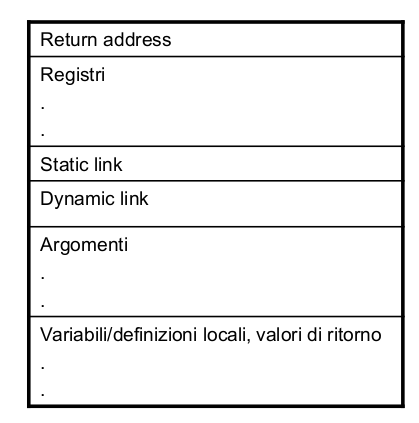
\includegraphics[scale=0.6]{img/act.png}
\end{center}
\newpage
Partiamo ora dal seguente codice in \textit{C}, e analizziamo i passaggi che avvengono nello stack:
\begin{minted}{C}
/* prima procedura */
int doppio(x) { 
	return 2 * x; 
}

/* seconda procedura, che chiama la prima */
int doppio_42(z) { 
	return doppio(z) - 42; 
}

/* chiamata nel main */
int r = doppio_42(42)
\end{minted} 
vediamo cosa accade nello stack:
si definiscono in ordine \textit{global frame e doppio\_42}, con i collegamenti di static link e dynamic link:
\begin{center}
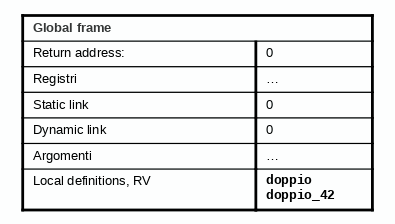
\includegraphics[scale=0.4]{img/sta1.png}
\quad 
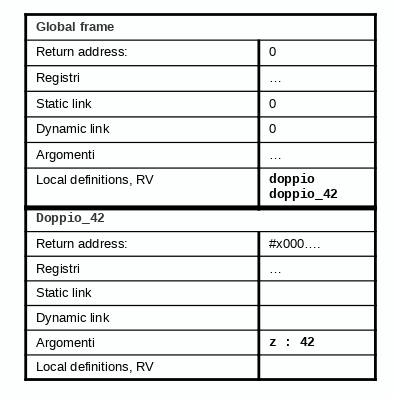
\includegraphics[scale=0.4]{img/sta2.png}
\quad
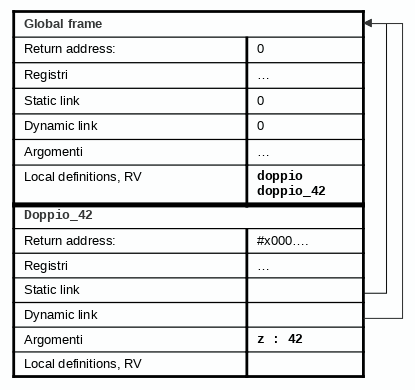
\includegraphics[scale=0.4]{img/sta3.png}
\end{center}
\newpage
Si aggiunge poi \textit{doppio}, con i collegamenti di static link e dynamic link:
\begin{center}
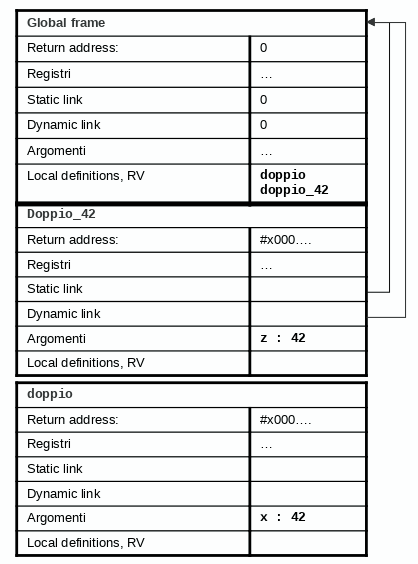
\includegraphics[scale=0.4]{img/sta4.png}
\quad 
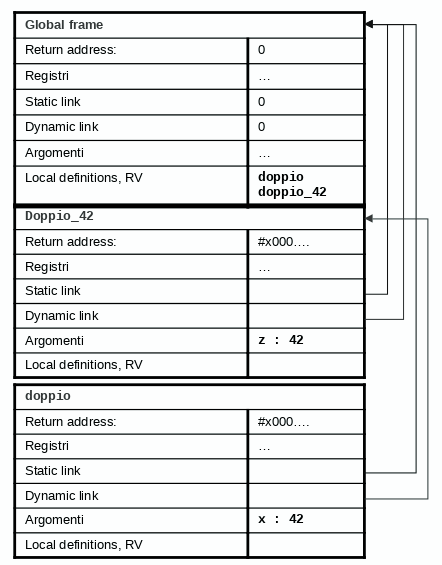
\includegraphics[scale=0.4]{img/sta5.png}
\end{center}
infine vengono risolti a partire da \textit{doppio}, salvando ogni volta i vari risultati nelle \textit{local definitions}:
\begin{center}
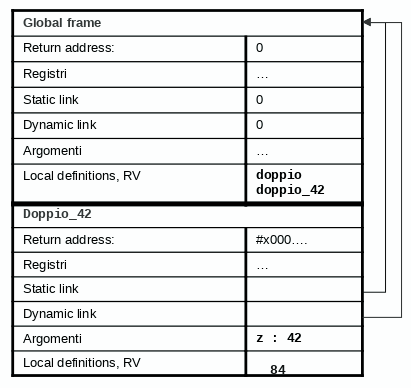
\includegraphics[scale=0.4]{img/sta6.png}
\quad
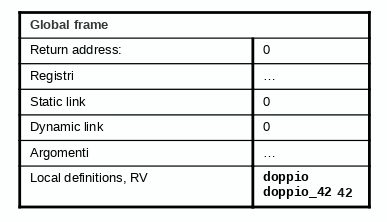
\includegraphics[scale=0.4]{img/sta7.png}
\end{center}
L'area di memoria per la manipolazione di strutture dati dinamiche verrà spiegata meglio al momento dell'introduzione delle primitive per la costruzione delle liste in Prolog e Lisp.\\
Il componente software che si occupa della gestione automatica della memoria in \textit{Lisp, Prolog, Java, C\#}, ed altri linguaggi è il \textit{garbage collector} (il servizio di raccolta rifiuti). \textit{C} e \textit{C++} non hanno un garbage collector standard.
\section{Logica}
Si ricordano le seguenti due definizioni:
\begin{enumerate}
\item \textbf{Implicazione}, indicata dal simbolo $\to$, è un connettivo logico che si usa per costruire forme logiche complesse. In una frase il \textit{se} comporta un'implicazione logica.
\item \textbf{Inferenza} è un meccanismo per il ragionamento. Detta anche \textit{modus ponens}, è una manipolazione sintattica (quindi non rappresentabile con tabelle di verità)
\end{enumerate}
Partiamo con l'esempio di una semplice dimostrazione geometrica effettuata con le regole della logica:
\begin{teorema}
Dato un triangolo isoscele (con $\overline{AB}=\overline{BC}$) si ha che $\angle A$, ovvero l'angolo in $A$, e $\angle C$, ovvero l'angolo in $C$, sono uguali.
\begin{center}
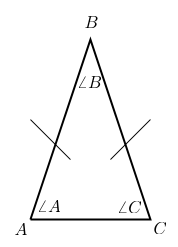
\includegraphics[scale=0.5]{img/tri.png}
\end{center}
\end{teorema}
\begin{proof}
Si comincia la dimostrazione con l'elenco delle conoscenze pregresse: 
\begin{enumerate}
\item se due triangoli sono uguali essi hanno lati e angoli uguali
\item se due triangoli hanno due lati e l'angolo sotteso uguale allora i due triangoli sono uguali
\item se viene definita la bisettrice di $\angle B$, $\overline{BH}$, si ha che $\angle ABH = \angle HBC$
\begin{center}
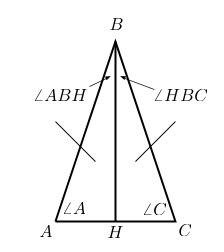
\includegraphics[scale=0.5]{img/tri2.png}
\end{center}
\end{enumerate}
Procediamo ora coi passi della dimostrazione:
\begin{enumerate}
\item $\overline{AB}=\overline{BC}$ per ipotesi
\item $\angle ABH = \angle HBC$ per la terza conoscenza pregressa
\item $\triangle HBC = \triangle ABH$ per la seconda conoscenza pregressa (dal secondo passo si ha che l'angolo tra la bisettrice, per forza uguale tra i due triangoli, e i due lati obliqui, uguali per ipotesi, è uguale per entrambi)
\item $\angle A= \angle C$ per la prima conoscenza pregressa (essendo uguali i triangoli per il passo precedente si ha che anche gli angoli sono uguali)
\end{enumerate}
Siamo così giunti alla fine della dimostrazione. Bisogna ora rappresentarla con gli strumenti della logica.\\
Sono stati svolti i seguenti passaggi:
\begin{itemize}
\item si è trasformata la seconda conoscenza pregressa in:\\\textbf{se} $\overline{AB}=\overline{BC}$ \textbf{e} $\overline{BH}=\overline{BH}$ \textbf{e} $\angle ABH = \angle HBC$ \textbf{allora} $\triangle ABH=\triangle HBC$
\item si è trasformata la prima conoscenza pregressa in:\\
\textbf{se} $\triangle ABH=\triangle HBC$ \textbf{allora} $\overline{AB}=\overline{BC}$ \textbf{e} $\overline{BH}=\overline{BH}$ \textbf{e} $\overline{AH}=\overline{HC}$ \textbf{e} $\angle ABH = \angle HBC$ \textbf{e} $\angle AHB = \angle CBH$ \textbf{e} $\angle A=\angle C$
\end{itemize}
Possiamo ora procedere col processo di \textbf{formalizzazione}, ovvero razionalizzare il processo per poter affermare:
$$\overline{AB}=\overline{BC}\,\vdash \angle A = \angle C$$
con $\vdash$ che è il simbolo di \textit{derivazione logica} e significa "consegue", "allora" etc...\\
Quindi per ottenere:
$$\overline{AB}=\overline{BC}\,\vdash \angle A = \angle C$$
abbiamo assunto:
$$P=\{\overline{AB}=\overline{BC},\,\angle ABH = \angle HBC,\,\overline{BH}=\overline{BH}\}$$
con queste conoscenze pregresse:
\begin{enumerate}
\item $\overline{AB}=\overline{BC}\wedge\overline{BH}=\overline{BH}\wedge\angle ABH = \angle HBC\to\triangle ABH=\triangle HBC$
\item  $\triangle ABH=\triangle HBC\to\overline{AB}=\overline{BC}\wedge\overline{BH}=\overline{BH}\wedge\overline{AH}=\overline{HC}\wedge\angle ABH = \angle HBC\wedge\angle AHB = \angle CBH\wedge\angle A=\angle C$
\end{enumerate}
Si ha quindi una catena di formule (\textbf{P} sono le ipotesi iniziali):
\begin{enumerate}
\item \textbf{P1:} $\overline{AB}=\overline{BC}$ preso da \textbf{P}
\item \textbf{P2:} $\angle ABH = \angle HBC$ preso da \textbf{P}
\item \textbf{P3:} $\overline{BH}=\overline{BH}$ preso da \textbf{P}
\item \textbf{P4:} $\overline{AB}=\overline{BC}\wedge\overline{BH}=\overline{BH}\wedge\angle ABH = \angle HBC$ preso da \textbf{P1, P2, P3} e dalla regola di inferenza detta \textbf{introduzione della congiunzione}
\item \textbf{P5:} $\triangle ABH=\triangle HBC$ da \textbf{P4}, dalla \textbf{regola 2} (\textit{se due triangoli hanno due lati e l'angolo sotteso uguale allora i due triangoli sono uguali}) e dalla regola di inferenza detta \textbf{modus ponens}
\item \textbf{P6:} $\overline{AB}=\overline{BC}\wedge\overline{BH}=\overline{BH}\wedge\overline{AH}=\overline{HC}\wedge\angle ABH = \angle HBC\wedge\angle AHB = \angle CBH\wedge\angle A=\angle C$ da \textbf{P5}, dalla \textbf{regola 1} (\textit{se due triangoli sono uguali essi hanno lati e angoli uguali}) e dalla regola di inferenza detta \textbf{modus ponens}
\item \textbf{P7:} $\angle A=\angle C$ da \textbf{P6} e dalla regola d'inferenza detta \textit{eliminazione della congiunzione} (date più asserzioni collegate da $\wedge$ posso eliderne un numero a piacere)
\end{enumerate}
Abbiamo così dimostrato tutto anche per mezzo dei costrutti della logica
\end{proof}
\begin{definizione}
Una dimostrazione del tipo \textit{F è conseguenza di S}, \textbf{dim}, si indica con:
$$S\,\,\vdash\,\, F$$
ed è una sequenza:
$$dim=<P_1,P_2,...,P_n>$$
con:
\begin{itemize}
\item $P_n=F$
\item $P_i\in S$ o con $P_i$ ottenibile dalle $P_1,...,P_{i-1}$ applicando una regola di inferenza
\end{itemize}
\end{definizione}
Un insieme di regole di inferenza costituisce la base di un calcolo logico e diversi insiemi di regole danno vita a diversi calcoli logici. Un calcolo logico ha lo scopo di manipolare le formule in modo unicamente sintattico, stabilendo una connessione tra un'insieme di formule di partenza, dette \textit{assiomi}, e un insieme di conclusioni.
\subsection{Logica Proporzionale}
La logica proposizionale si occupa delle conclusioni che si possono trarre da un insieme di proposizioni, che definiscono \textit{sintatticamente} la logica proposizionale (l'ultima parte della dimostrazione sopra è fatta da costrutti della logica proposizionale).\\
All'insieme \textbf{P} è associata una funzione di \textit{verità}, o di \textit{valutazione}, \textbf{V} (spesso indicata con \textbf{T} o \textbf{I}):
$$V:P\to\{vero,\,\,falso\}$$
che associa un valore di verità ad ogni eleemnto di \textbf{P}. La funzione di valutazione è il ponte di connessione tra sintassi e semantica in un linguaggio logico.\\
Le proposizione si combinano con i seguenti connettivi:
\begin{itemize}
\item \textbf{congiunzione:} $\wedge$
\item \textbf{disgiunzione:} $\vee$
\item \textbf{negazione:} $\neg$
\item \textbf{implicazione:} $\to$
\end{itemize}
L'insieme di tutte le formule formate dagli elementi di \textbf{P} e dalle loro combinazioni è detto: \textbf{Formule Ben Formate (FBF)}.\\
Le formule atomiche e i loro negativi vengono detti \textbf{letterali}. Il valore di verità di proposizione dipende dalla funzione di verità \textbf{V} e questa definizione può essere estesa sul dominio \textbf{FBF}:
\begin{itemize}
\item $V(\neg s)=non\,V(s)$
\item $V(a\wedge b)=V(a)\,\ e\,\, V(b)$
\item $V(a\vee b)=V(a)\,\ o\,\, V(b)$
\item $V(a\to b)=(non\,V(a))\,\ o\,\, V(b)$
\end{itemize}
ovvero, secondo la tavola di verità (con $1=vero$ e $0=falso$):
\begin{center}
\begin{tabular}{|c|c|c|c|c|c|c|}
\hline
$a$ & $b$ & $\neg a$ & $\neg b$ & $a\wedge b$ & $a\vee b$ & $a\to b$\\
\hline
1 & 1 & 0 & 0 & 1 & 1 & 1\\
\hline
1 & 0 & 0 & 1 & 0 & 1 & 1\\
\hline
0 & 1 & 1 & 0 & 0 & 1 & 0\\
\hline
0 & 0 & 1 & 1 & 0 & 0 & 1\\
\hline
\end{tabular}
\end{center}
La tavola di verità costituisce la semantica di un insieme di proposizioni mentre un calcolo logico dice come generare nuove formule logiche, ovvero espressioni sintattiche, a partire dagli assiomi. Questo calcolo deve garantire che le nuove formule generate siano vere se gli assiomi sono veri. Questo processo di generazione si chiama \textbf{dimostrazione}.\\
Per ottenere nuove formule dagli assiomi si usa il calcolo proposizionale, che si base su regole di inferenza. Una regola di inferenza ha la seguente forma:
$$\frac{F_1,F_2,...,F_N}{R}\,\,[\mbox{nome regola}]$$
con $F_i$ formula vera in \textbf{FBF} e $R$ è la formula vera generata da inserire in \textbf{FBF}. Vediamo qualche esempio:
\begin{esempio}[Modus Ponens]
$$\frac{a\to b,\,\,a}{b}$$
ovvero:
\begin{itemize}
\item Se piove, la strada è bagnata
\item Piove
\item Allora la strada è bagnata
\end{itemize}
Ovvero, la regola sintattica del modus ponens ci permette di
aggiungere le conclusioni di una “regola” al nostro insieme di formule ben formate “vere”
\end{esempio}
\begin{esempio}[Modus Tollens]
$$\frac{a\to b, \neg b}{\neg a}$$
ovvero:
\begin{itemize}
\item Se piove, la strada è bagnata
\item La strada non è bagnata
\item Allora non piove
\end{itemize}
Ovvero, la regola sintattica del modus tollens ci permette di
aggiungere la premessa negata di una “regola” al nostro insieme di formule ben formate “vere”
\end{esempio}
\begin{esempio}[Eliminazione e Introduzione di $\wedge$]
$$\frac{P_1\wedge P_2 \wedge ... \wedge P_n}{P_i}\,\,[\mbox{Eliminazione di }\wedge]$$
ovvero:
\begin{itemize}
\item Piove e la strada è bagnata
\item Piove
\end{itemize}
$$\frac{P_1, P_2,...,P_n}{P_1\wedge P_2 \wedge ... \wedge P_n}\,\,[\mbox{Introduzione di }\wedge]$$
ovvero:
\begin{itemize}
\item Piove
\item La strada è bagnata
\item Piove e la strada è bagnata
\end{itemize}
Ovvero, la regola sintattica dell’eliminazione della congiunzione ci permette di aggiungere all’insieme \textbf{FBF} i singoli componenti di una formula complessa. \\
Queste regole si chiamano anche, rispettivamente, \textit{di congiunzione} e \textit{di disgiunzione}
\end{esempio}
\begin{esempio}[Introduzione di $\vee$]
$$\frac{a}{a\vee b}$$
ovvero:
\begin{itemize}
\item Piove
\item Piove o c'è vita su Marte
\end{itemize}
Ovvero, la regola sintattica dell’introduzione della disgiunzione ci permette di aggiungere i singoli componenti di una formula.\\
Questa regola è detta anche \textit{di addizione}
complessa
\end{esempio}
\begin{esempio}
Ecco altre regole utili:
\begin{itemize}
\item \textbf{Terzo Escluso:}
$$\frac{a\vee\neg a}{vero}$$
\item \textbf{Eliminazione di} $\neg$:
$$\frac{\neg\neg a}{a}$$
\item \textbf{Eliminazione di} $\wedge$:
$$\frac{a\wedge vero}{a}$$
\item \textbf{Contraddizione:}
$$\frac{a\wedge\neg a}{b}$$
ovvero da una contraddizione posso trarre qualsiasi conseguenza
\end{itemize}
\end{esempio}
Queste regole di inferenza fanno parte del \textit{calcolo naturale}, detto anche \textit{di Gentzen}, ovvero il loro formalizzatore. Questo tipo di calcolo consiste nel formalizzare i modi di derivare conclusioni a partire dalle premesse, ovvero di derivare direttamente un FBF mediante una sequenza di passi ben codificati. La regola del \textit{modus ponens} (ovvero l'eliminazione dell'implicazione), insieme al principio del terzo escluso, posso essere usati anche \textit{procedendo per assurdo} alla dimostrazione di una data formula; questa procedura è detta \textit{principio di risoluzione}. Il \textit{principio di risoluzione} è una regola di inferenza generalizzata semplice e facile da utilizzare e implementare. Questo principio lavora su FBF trasformate in \textit{forma normale congiunta}, dove ogni congiunto è detto \textit{clausola}. L'osservazione alla base del principio è un'estensione della rimozione dell'implicazione sulla base del principio di contraddizione e si usa per dimostrazioni per assurdo:
$$\frac{p\vee r,\, s\vee r}{p\vee s}\,\,\,\,\,\,\,\,\,\,\frac{\neg r,\, r}{\perp}$$
dove:
\begin{itemize}
\item $p\vee s$ è la \textit{clausola risolvente}
\item $\perp$ è la \textit{clausola vuota}, che corrisponde all'aver creato una contraddizione con delle FBF (posso infatti dedurre qualsiasi cosa, anche la clausola vuota)
\end{itemize}
\newpage
vediamo un'altra regola di inferenza:
\begin{esempio}[(unit) resolution]
$$\frac{\neg p,\,\, q_1\vee q_2\vee ... \vee q_k \vee p}{q_1\vee q_2\vee ... \vee q_k}$$
o anche:
$$\frac{p,\,\, q_1\vee q_2\vee ... \vee q_k \vee \neg p}{q_1\vee q_2\vee ... \vee q_k}$$
è una regola di risoluzione molto generale e se una delle due clausole da risolvere è un \textit{letterale} (come negli esempi) si parla di \textit{unit resolution}. Come esempio di può avere:
\begin{itemize}
\item non piove, piove e c'è il sole
\item c'è il sole
\end{itemize}
\end{esempio}
Vediamo ora come funzionano le dimostrazioni per assurdo.\\
Si supponga di avere un'insieme di FBF vere e di avere una proposizione \textit{p} da dimostrare vera. Si ha il metodo \textit{reductio ad absurdum}:
\begin{itemize}
\item assumo $\neg p$ vera
\item se combinandola con le FBF ottengo una contraddizione allora $p$ deve essere vera (o meglio derivabile)
\end{itemize}
\begin{esempio}[provo che q è vera]
assumo:
\begin{itemize}
\item $FBF=\{p\to q,\,\,p,\,\,\neg w,\,\,e,\,\,r\}$
\item assumo vera $\neg q$
\end{itemize}
si ha che $FBF\cup \{\neg q\}$ genera una contraddizione infatti:
\begin{itemize}
\item $p\to q \equiv\neg p\vee q$ combinato con $p$ produce $q$ e quindi si ha $q\vee\neg q$, ovvero una contraddizione
\item se applico a $q$ e $\neg q$ il principio di risoluzione ottengo la clausola vuota $\perp$
\end{itemize}
\end{esempio}
Torniamo ad analizzare gli assiomi. Si hanno delle proposizioni sempre vere:
\begin{itemize}
\item $a\to(b\to a)$
\item $(a\to(b\to c))\to((a\to b)\to(a\to c))$
\item $(\neg b\to \neg a)\to ((\neg b\to a)\to b)$
\item $\neg(a\wedge \neg a)$ detto \textit{principio di non contraddizione}
\item $a\vee \neg a$ detto \textit{principio} del terzo escluso
\end{itemize}
Vediamo un esempio:
\begin{esempio}
Si ha la seguente affermazione:\\
\textit{se l'unicorno è mitico, allora è immortale, ma se non è mitico allora è mortale. Se è mortale o immortale, allora è cornuto. L'unicorno è magico se è cornuto.} Ho le seguenti domande:
\begin{enumerate}
\item l'unicorno è mitico?
\item l'unicorno è magico?
\item l'unicorno è cornuto?
\end{enumerate}
Bisogna quindi esprimere il problema con la logica delle proposizioni, individuare teoremi da dimostrare e infine dimostrarli. Le proposizioni saranno quindi:
\begin{itemize}
\item UM = unicordo è mitico
\item UI = unicorno è immortale
\item UMag = unicorno è magico
\item UC = unicorno è cornuto
\end{itemize}
che trascritto in logica diventa, che sono le mie conoscenze pregresse:
$$UM\to UI$$
$$\neg UM \to \neg UI$$
$$\neg UI\vee UI\to UC$$
$$UC\to Umag$$
dimostro ora le domande rappresentandole in forma logica. Si ha:
$$S=\{UM\to UI,\,\,\neg UM \to \neg UI,\,\,\neg UI\vee UI\to UC,\,\,UC\to Umag\}$$
con le domande che diventano:
\begin{itemize}
\item $S\vdash UM$?
\item $S\vdash Umag$?
\item $S\vdash UC$?
\end{itemize}
\newpage
Inizio a dimostrare la terza:\\
$$P1: \neg UI\vee UI\to UC\,\, \mbox{ da }S$$
$$P2: \neg UI\vee UI \mbox{ da }A5 \mbox{(tautologia)}$$
$$P3: UC\mbox{ da}P2,\,P2\,\, e\,\, ModusPonens$$
$P3$ si può scrivere già perché $P2$ è una tautologia, quindi posso utilizzare il modus ponens.\\
Ecco la seconda:\\
$$P4: UC\to Umag \mbox{ da }S$$
$$P5: Umag \mbox{ da }P3,\,P4\,\, e\,\, ModusPonens$$
Ed ecco la prima:\\
non è dimostrabile con queste conoscenze pregresse, non posso usare nessuna regola di inferenza
\end{esempio}
Si hanno differenze tra \textit{sintassi} e \textit{semantica}. L'operazione di derivazione $\vdash$ è un operatore sintattico e il calcolo logico fornisce una manipolazione sintattica e simbolica.\\ 
La semantica dipende dalla funzione di interpretazione, o funzione di valutazione o funzione di verità, $V$, che si basa sulle tabelle di verità. Si ha l'operatore di \textit{conseguenza logica} $\models$. Si ha, data una particolare logica che:
$$S\vdash f \mbox{ se e solo se } S\models f$$
Con $S$ insieme di formule iniziale e $f$ una FBF, il tutto in dipendenza da una funzione di verità $V$.\\
Una FBF vera indipendentemente dai valori dei letterali è detta \textit{tautologia}. Una particolare interpretazione $V$ che rende vere tutte le formule di $S$ è detta \textit{modello} di $S$.
\newpage
\subsection{Logica del primo ordine}
Di cui fanno parte i sillogismi (tutti gli uomini sono mortali, Socrate è mortale quindi Socrate è mortale). Si ha la \textit{logica proposizionale}, computazionalmente e semanticamente più chiara, ma limitata nella difficoltà di rappresentare asserzioni circa insiemi di elementi in maniera concisa. Nel sillogismo sopra la prima frase non è esprimibile in logica proposizionale. Si hanno le seguenti nozioni nella logica del primo ordine (LPO):
\begin{itemize}
\item variabile
\item costante
\item relazione (o predicato), che è un sottoinsieme di un prodotto cartesiano
\item funzione
\item quantificatore
\end{itemize}
quindi un linguaggio del primo ordine è costituito da \textit{termini} costruiti a partire da:
\begin{itemize}
\item \textit{V} insieme di simboli di variabili
\item \textit{C} insieme di simboli di costante
\item \textit{R} insieme di simboli di relazione o predicati di varia arità
\item \textit{F} insieme fi funzioni di varia arità
\item connettivi logici e simboli di quantificazione universale, $\forall$ (universale, "per ogni") e $\exists$(esistenziale, "esiste")
\end{itemize}
La costruzione di un linguaggio di primo ordine è \textit{ricorsiva}. I termini più semplici sono predicati
$$r\subseteq C_0\times C_1\times\cdots\times C_n$$
ovvero le relazioni cartesiane su \textit{C}, scritte come $r(c_1,...,c_n)$.\\
Le funzioni sono definite con dominio e codominio:
$$f:C_0\times C_1\times\cdots\times C_n\to C$$
e una funzione si scrive come $f(c_1,...,c_n)$.\\
Si hanno FBF costruite ricorsivamente da:
\begin{itemize}
\item un \textit{termine}, ovvero un elemento di \textit{C}, \textit{V} o l'applicazione di una funzione $f(t_1,t_2,...t_n)$
\item un termine costruito da un predicato $r(t_1,t_2,...t_n)$, con $t_i$ termini, appartiene ad una FBF
\item diversi elementi di FBF connessi da connettivi logici standard($\vee,\,\wedge,\,\neg,\,\to$) appartengono a FBF, tali combinazioni sono dette $t(t_1,t_2,...t_n)$
\item le formule $\forall x,\,t(t_1,t_2,...t_n)$ e $\exists x,\,t(t_1,t_2,...t_n)$ appartengono a FBF
\end{itemize}
Rivediamo ora il sillogismo \textit{tutti gli uomini sono mortali, Socrate è mortale quindi Socrate è mortale}. Ho:
\begin{itemize}
\item l'insieme delle costanti individuali $C=\{Sorate,\, Platone,\,...\}$
\item l'insieme dei predicati $P=\{uomo,\,mortale\}$
\end{itemize}
traduco quindi le asserzioni principali del sillogismo:
$$\forall x, (uomo(x)\to mortale(x))$$
$$uomo(Socrate)$$
e traduco la conclusione:
$$mortale(socrate)$$
Bisogna giustificare la semantica con nuove regole.\\
Si aggiunge una nuova regola d'inferenza per la logica dei predicati, l'eliminazione del quantificatore universale $\forall$ (\textit{C} insieme delle costanti):
$$\frac{\forall x, T(...,x,...), c\in C}{T(...,c,...)}$$
Quindi risolvo il sillogismo con questa regola:
$$\frac{(\forall x, uomo(x)\to mortale(x)), Socrate\in C}{uomo(Socrate)\to mortale(Socrate)}$$
poi applico il modus ponens, detto, per la logica proposizionale, anche \textit{eliminazione dell'implica} $\to$:
$$\frac{uomo(Socrate), uomo(Socrate)\to mortale(Socrate)}{mortale(Socrate)}$$
Abbiamo altre regole di inferenza per il quantificatore esistenziale:
\begin{itemize}
\item Introduzione del quantificatore esistenziale $\exists$:
$$\frac{T(...,c,...), c\in C}{\exists x, T(...,x,...)}$$
\item si hanno le seguente identità:
$$\exists x, \neg T(...,x,...)\equiv \neg\forall x, T)...,x,...)$$
$$\forall x, \neg T(...,x,...)\equiv \neg\exists x, T(...,x,...)$$
\end{itemize}
\chapter{Prolog}
Il prolog è un linguaggio logico rappresentato da una semplicità del formalismo, è di alto livello e ha una semantica chiara. Un programma è un insieme di formule e si ha come fine la dimostrazione di un'affermazione. La base formale è data dalle \textit{clausole di Horn} e dal meccanismo di \textit{risoluzione}. Prolog viene da \textit{PROgramming LOGic} e si basa su una restrizione della logica del primo ordine e usa uno stile dichiarativo. Si vuole determinare la veridicità di una affermazione. Ogni FBF può essere in \textit{forma normale a clausola}:
\begin{itemize}
\item \textit{formula normale congiunta:} congiunzione di disgiunzioni o di negazione di predicati (sia positivi che negativi):
$$\wedge_i(\vee_iL_{ij})$$
\begin{esempio}
ecco degli esempi:
\begin{itemize}
\item $(p(x)\vee q(x,y)\vee \neg t(z))\wedge(p(w)\vee\neg s((u)\vee \neg r(v))$
\item $(\neg t(z))\vee (p(w)\vee\neg s(u))\wedge (p(x)\vee s(x)\vee q(y))$
\end{itemize}
che sono riscrivibili come:
$$t(z)\to p(x)\vee q(x,y)$$
e
$$s(u)\wedge r(v)\to p(w)$$
\end{esempio}
\item \textit{forma normale disgiunta}: disgiunzione di congiunzioni o di negazione di predicati (sia positivi che negativi)
$$\vee_i(\wedge_iL_{ij})$$
\end{itemize}
Le clausole con un solo letterale positivo solo le \textit{clausole di Horn} e un programma in prolog è una collezione di \textit{clausole di Horn}. Non tutte le FBF possono essere \textit{clausole di Horn}.\\
Prolog non ha istruzioni. Si hanno \textit{fatti} (asserzioni vere nel contesto descritto) e \textit{regole}.\\
%aggiungi roba
Parliamo di sintassi:
\begin{itemize}
\item ":-" è l'implicazione
\item tutto termina con un punto "."
\item la "," è l'and logico
\item il ";" è lor logico
\item \textit{a.} è un fatto o asserzione
\item \textit{b :- c, d, ... .} è una regola (c, d, ... termini composti)
\item \textit{? :- x, y, ... .} è un goal o una query (x, y, ... termini composti)
\item non si dichiarano variabili e si ha solo la lista come struttura dati. SI hanno vari termini (atomi variabili etc...):
\begin{itemize}
\item atomi (numeri, ...) ovvero caratteri alfanumerici che inizia col carattere minuscolo (puo esserci \_ ma quindi non un numero), qualsiasi cosa dentro apici "" o numeri.
\item variabili è un carattere che inizia con la maiuscola (e quindi non con un numero) o col carattere \_ (che indica una variabile anonima o \textit{indifferenza}). Le variabili si istanziano (non con un assegnamento) col procedere del programma e della dimostrazione
\item termine composto (col simbolo +). Un \textit{funtore} è un simbolo di funzione o predicato che applica ad argomenti, messi tra parentesi tonde (da non spaziare dal funtore). Il funtore è minuscolo e non è un numero
\end{itemize}
\item un \textit{fatto} è un nome di predicato che inizia con la maiuscola
\item una \textit{regola} esprime la dipendenza di un fatto da un insieme di altri fatti. Possono esprimere anche definizioni
\item una regola ha una \textit{testa (head)}, ed è il conseguente e un \textit{corpo (body)}, l'antecedente. Si ha quindi un solo termine come conseguente (\textit{regola di Horn}). Si ha quindi:
\textit{un pesce è un animale e ha le squame}: 
\begin{minted}{prolog}
pesce(x) :- animale(x), ha_le_squame(x).
\end{minted}
%oppure:\\
%\textit{gigi ama chiunque ami il vino}
%aggiungi prolog
\item una relazione si può esprimere con più regole:
\begin{minted}{prolog}
genitore(x, y) :- padre(x,y).
genitore(x, y) :- madre(x,y).
\end{minted}
\item si ha la ricorsione per definire una relazione. La definizione richiede almeno due proposizioni, \textit{caso base} e \textit{caso generale}:
\begin{minted}{prolog}
antenato(x, y) :- genitore(x, y).
antenato(x, y) :- genitore(z, y), antenato(x, z).
\end{minted}
\item i commenti in linea si hanno con \% e su più linee con /* e */
\begin{minted}{prolog}
%commento
antenato(x, y) :- genitore(x, y).
antenato(x, y) :- genitore(z, y), antenato(x, z).
/*commento
su più righe*/
\end{minted}
\item il prompt ci chiede una FBF di Horn con "?-" (senza variabili) e prende l'input e come output si avrà \textit{yes}. Interrogare il programma è richiedere una dimostrazione. Se si chiede una formula presente direttamente si avrà subito \textit{yes} (se il goal è una clausola (un fatto) quindi si applica il principio di risoluzione e si ha la dimostrazione effettuata). In un'interrogazione si possono avere \textit{variabili esistenziali}. Tutte le variabili istanziate sono mostrate in risposta
\item l'operatore di istanziazione di variabili durante la prova di un predicato è il risultato di una procedura particolare, detta \textit{unificazione}
\item dati due termini la procedura di unificazione crea un insieme di sostituzioni delle variabili. Questo insieme permette di rendere uguali i due termini. Tradizionalmente si ha il \textit{most general unifier (Mgu)}. Una sostituzione è indicata come una sequenza ordinata di coppie \textit{variabile/valore}:
\begin{minted}{prolog}
Mgu(42, 42) % ->{} non serve nessuna sostituzione
Mgu(42, X) % ->{X/42} ovvero X deve essere 42
Mgu(X,42) % ->{X/42} ovvero X deve essere 42
Mgu(foo(bar, 42), foo(bar, X)) % ->{X/42} ovvero X deve essere 42
Mgu(foo(X, 42), foo(bar, X)) % ->{Y/bar, X/42} ovvero X deve essere 42

Mgu(foo(bar(42), baz), foo(X, Y))  /* ->{X/bar (42), Y/baz}
 ovvero X deve essere  bar(42) e Y baz*/
Mgu(foo(X), foo(bar(Y))) 
Mgu(foo(bar(42), baz), foo(X, Y))  /* ->{X/bar (y), Y_:G001}
 ovvero non si ha soluzione */
\end{minted}
L'Mgu non è altro che il risultato finale della procedura di valutazione del Prolog. Il modo più semplice per vedere se l'unificazione funziona è usare "=", ovvero, ricollegandoci al codice sopra:
\begin{minted}{prolog}
?- 42 = 42.
Yes

?- 42 = X.
X = 42 % per rendere vera l'affermazione serve x = 42
Yes

?- foo(bar, 42) = foo(bar, X).
X = 42
Yes

?- foo(Y, 42) = foo(bar, X).
Y = bar
X = 42
Yes

?- foo(bar(42), baz) = foo(X, Y).
X = bar(42)
Y = baz
Yes

?- foo(X) = foo(bar(Y)).
X = bar(Y)
Y = _G001
Yes

?- foo(42, bar(X), trillian) = foo(Y, bar(Y), X).
No
\end{minted}
\begin{esempio}
\textit{Si descrive un insieme di fatti riguardanti i corsi offerti:}\\
Tutte le informazioni sono concentrate in una relazione a 6 campi:
\begin{minted}{prolog}
corso(linguaggi, lunedì, ’9:30’, ’U4’, 3, antoniotti).
corso(biologia_computazionale, lunedì, ’14:30’, ’U14’, t023, antoniotti).
\end{minted}
a partire da qui costruisco altri predicati:
\begin{minted}{prolog}
aula(Corso, Edificio, Aula) :-
	corso(Corso, _, _, Edificio, Aula, _).
docente(Corso, Docente) :-
	corso(Corso, _, _, _, _, Docente).
\end{minted}
oppure posso concentrare le informazioni in una relazione con 4 campi; le informazioni sono concentrate in termini funzionali che rappresentano le informazioni raggruppate logicamente;
\begin{minted}{prolog}
corso(linguaggi, orario(lunedì, ’9:30’), aula(’U4’, 3), antoniotti).
corso(biologia_computazionale,
	orario(lunedì, ’14:30’),
	aula(’U4’, 3),
	antoniotti).
\end{minted}
posso quindi definire altri predicati:
\begin{minted}{prolog}
aula(Corso, Edificio, Aula) :- corso(Corso, _, aula(Edificio, Aula), _).
docente(Corso, Docente) :- corso(Corso, _, _, Docente).

% oppure...

aula(Corso, Luogo) :- corso(Corso, _, Luogo, _).
\end{minted}
oppure ancora i predicati che abbiamo definito a partire dalle relazioni con 6 o 4 campi possono essere ricodificate con predicati binari:
\begin{minted}{prolog}
giorno(linguaggi, martedì).
orario(linguaggi, ’9:30’).
edificio(linguaggi, ’U4’).
aula(linguaggi, 3).
docente(linguaggi, antoniotti).
\end{minted}
La relazioni a 6 o 4 argomenti possono essere ricostruite in a partire da queste relazioni binarie. La costruzione di schemi \textit{RDF/XML} (e, a volte,\textit{ SQL}) corrisponde a questa operazione di ri-rappresentazione
\end{esempio}
\item Si definisce una lista in Prolog racchiudendo gli elementi (termini e/o variabili logiche) della lista tra parentesi quadre \textit{[} e \textit{]} e separandoli da virgole. Gli elementi di una lista in Prolog possono essere termini
qualsiasi o liste. La lista vuota si indica con \textit{[]}. Una coda non vuota si può dividere in \textit{testa} e \textit{coda}:
\begin{itemize}
\item la testa è il primo elemento della lista
\item la coda rappresenta tutto il resto ed è sempre una lista
\end{itemize}
\begin{minted}{prolog}
[a, b, c] % a è la testa e [b, c] la coda
[a, b] % a è la testa e [b] la coda
[a] % a è la testa e [] la coda
[[a]] % [a] è la testa e [] la coda
[[a, b], c] % [a, b] è la testa e [c] la coda
[[a, b], [c], d] % [a, b] è la testa e [[c], d] la coda
\end{minted}
Prolog possiede uno speciale operatore usato per distinguere tra l'inizio e la coda di una lista: l'operatore \textit{|}:
\begin{minted}{prolog}
?- [X | Ys] = [mia, vincent, jules, yolanda].
X = mia
Ys = [vincent, jules, yolanda]
Yes

?- [X, Y | Zs] = [the, answer, is, 42].
X = the
Y = answer
Zs = [is, 42]
Yes

?- [X, 42 | _] = [41, 42, 43, foo(bar)].
X = 41
Yes
\end{minted}
La lista vuota \textit{[]} in prolog è gestita come una lista speciale:
\begin{minted}{prolog}
?- [X | Ys] = [].
No
\end{minted}
\item La base di conoscenza è nascosta ed è accessibile solo tramite opportuni comandi o tramite ambiente di programmazione. Bisogna poter caricare un insieme di fatti e regole. Per farlo si ha il comando \textit{consult}, che appare come un predicato da valutare (un goal) e prende almeno un termine che denota un file come argomento, file che deve contenere fatti e regole
\begin{minted}{prolog}
?- consult(’guida-astrostoppista.pl’).
Yes

?- consult(’Projects/Lang/Prolog/Code/esempi-liste.pl’).
Yes
\end{minted}
\item il predicato \textit{consult} può essere usato anche per inserire fatti e regole direttamente alla console usando il termine speciale \textit{user}:
\begin{minted}{prolog}
?- reconsult(’guida-astrostoppista.pl’).
Yes
% A questo punto la base di dati Prolog contiene il
% nuovo contenuto del file.
\end{minted}
il predicato \textit{reconsult} deve invece essere usato quando si vuole ricaricare un file (ovvero un data o knowledge base) nell'ambiente Prolog. L’effetto è di prendere i predicati presenti nel file, rimuoverli completamente dal data base interno e di reinstallarli utilizzando le nuove definizioni:
\begin{minted}{prolog}
?- reconsult(user). % Notare il sotto-prompt.
|- foo(42).
|- friends(zaphod, trillian).
|- ^D
Yes

% A questo punto la base di dati Prolog contiene i due
% fatti inseriti manualmente.
?- friends(zaphod, W).
W = trillian
Yes
\end{minted}
\item Prolog lavora anche su strutture ad albero e anche i programmi sono strutture dati manipolabili con predicati \textit{extra-logici}. Si ha la ricorsione e non l'assegnamento. Un programma Prolog è un insieme di clausole di Horn che rappresentano:
\begin{itemize}
\item fatti riguardanti gli oggetti in esame e le relazioni che intercorrono tra di loro
\item regole sugli oggetti e sulle relazioni (se ... allora ...)
\item interrogazioni (goals o queries; clausole senza testa), sulla base della conoscenza definita
\end{itemize}
\item si ha l'implicazione: 
$$\neg B \vee A \mbox{ corrisponde a } B\to A$$
data una clausola $A\vee ... \vee A_n\vee \neg B_1\vee ... \vee\neg B_n$, usando De Morgan si ottiene:
$$(A\vee ... \vee A_n)\vee \neg (B_1\vee ... \vee B_n)$$
$$\downarrow$$
$$(B\vee ... \vee B_n)\to (A_1\vee ... \vee A_n)$$
\textit{si può fare anche l'inverso}.\\
\end{itemize}
vediamo un programma che fa la somma tra due naturali:
\begin{minted}{prolog}
sum(0, X, X).
sum(s(X), y, s(Z)) -: sum(X, Y, Z).
\end{minted}
con $S(n)$ interpretato come il successore ($0=0,\, s(0)=1, \,s(s(0))=2,... $).\\
Quando viene specificato un goal esso viene confrontato con tutte le clausole di programma, che usa il procedimento di negazione e di trasformazione in sintassi Prolog.\\
Vediamo i passi:
\begin{itemize}
\item  interroghiamo il programma:
$$\exists X\,\,\, sum(s(0),\, 0,\, X)\,\,\,\,\,\{X\,/\, s(0)\}$$
$$\exists W\,\,\, sum(s(s(0)),\, s(0), \, W)\,\,\,\,\,\{W\,/\, s(s(s(0)))\}$$
dove $\{X\,/\, s(0)\}$ e $\{W\,/\, s(s(s(0)))\}$ sono le sostituzioni che rappresentano il risultato
\item usiamo il procedimento di negazione e trasformazione in sintassi:
\begin{minted}{prolog}
:- sum(s(0), 0, N).    %{N / s(0)}
:- sum (s(s(0)), s(0), W).     %{W / s(s(s(0)))}
\end{minted}
con $\{N\, /\, s(0)\}$ e $\{W \,/\, s(s(s(0)))\}$ che sono le \textbf{sostituzioni}. Una sostituzione ci dice che valori (che possono essere altre variabili) si può sostituire le variabili di un termine. Una sostituzione si indica con $\sigma=\{X_1\,/\,V_1/,..., X_k\,/\,V_k\}$ e può essere considerata come una funzione ($\sigma: T\to T$) applicabile ad un termine dell'insieme dei termini $T$.
\begin{esempio}
data la sostituzione $\sigma=\{X\,/\,42,\,Y\,/\, foo(s(0))\}$ si ha:
$$\sigma(bar(X,\,Y))=bar(42, \, foo(s(0)))$$
\end{esempio}
\end{itemize}
\newpage
\textit{Una computazione corrisponde al tentativo di dimostrare, tramite la regola di risoluzione, che una formula segue logicamente da un programma (è un teorema)}. Si ha inoltre che si deve determinare una sostituzione per le variabili del goal (le \textit{query}) per cui la query segue  logicamente dal programma:
\begin{esempio}
Sia dato il programma P e la query:
\begin{minted}{prolog}
:- p(t1, t2, ..., tm).
\end{minted}
se \textbf{X1,..., Xn} sono le variabili in \textbf{t1,..., tm}, il significato della query è:
$$\exists X1,\,..., \,Xn\, . \,p(t1, t2, ..., tm)$$
e si cerca una sostituzione:
$$s=\{X1\,/\,s1,...,\, Xn\,/\,sn$$
con gli $s\,i$ termini tali per cui:
$$P\vdash s[p(t1, t2, ..., tm)]$$
\end{esempio}
Dato un insieme di clausole di Horn è possibile derivare la clausola vuota solo se c'è almeno una clausola senza testa, ovvero se si ha una query $G_0$ da provare. Ovvero si deve dimostrare che da $P\cup G_0$ si può derivare la clausola vuota. Si dimostra per assurdo col principio di risoluzione.
\subsubsection{Risoluzione ad Input Lineare (SLD)}
Il sistema Prolog dimostra la veridicità di un goal eseguendo una sequenza di passi di risoluzione (l'ordine con cui vengono eseguiti questi passi rende i sistemi di prova basati sulla risoluzione più o meno efficienti). In Prolog la risoluzione avviene sempre fra l’ultimo goal derivato in ciascun passo e una \textit{clausola di programma} e mai fra due clausole di programma o fra una clausola di programma ed un goal derivato in precedenza. Questa forma di risoluzione è detta\textit{Risoluzione-SLD}  (\textit{Selection function for Linear and Definite sentences Resolution}), dove le sentenze lineari sono le clausole di Horn.
\begin{esempio}
partiamo dal goal $G_i$:
$$G_i\equiv \,\,\,?-\, A_{i,\, 1}, ...,  A_{i,\, m}.$$
e dalla regola:
$$A_r\,\,\,:-\,\,\, B_{r,\,1},..., B_{r,\,k}.$$
se esiste un unificatore $\sigma$ tale che $\sigma[A_r]=\sigma[A_{i,\,1}]$ allora si ottiene il nuovo goal:
$$G_{i+1}\equiv\,\,\,B^{'}_{r,\,1},..., B^{'}_{r,\,k},A^{'}_{i,\, 1}, ...,  A^{'}_{i,\, m}.$$
che è un passo di risoluzione eseguito dal sistema Prolog (con $\sigma[A_{i,\,m}]=A^{'}_{i,\,m}$ 4 $\sigma[B_{i,\,m}]=B^{'}_{i,\,m}$. \textit{La scelta di unificare il primo sottogoal di }$G_i$\textit{ è arbitraria (si sarebbe potuto scegliere, per esempio} $A_{i,\,m}$ \textit{o} $A_{i,\,c}$ \textit{con} $ c\in[1,\,m]$ \textit{)}
\end{esempio}
\begin{esempio}
partiamo dal goal $G_i$:
$$G_i\equiv \,\,\,?-\, A_{i,\, 1}, ...,  A_{i,\, m}.$$
e dalla regola (ovvero dal \textbf{fatto}):
$$A_r.$$
se esiste un unificatore $\sigma$ tale che $\sigma[A_r]=\sigma[A_{i,\,1}]$ allora si ottiene il nuovo goal:
$$G_{i+1}\equiv\,\,\,A^{'}_{i,\, 2}, ...,  A^{'}_{i,\, m}.$$
che ha dimensioni minori di $G_i$ avendo $m-1$ sottogoal
\end{esempio}
Nella risoluzione SLD, il passo di risoluzione avviene sempre fra l'ultimo goal e una clausola di programma. SI possono avere i seguenti risultati:
\begin{itemize}
\item \textbf{successo:} si genera la clausola vuota, ovvero se per $n$ finito $G_n$ è uguale alla clausola vuota $G_:n\equiv\,\,\,:-$
\item \textbf{insuccesso finito}: se per $n$ finito $G_n$  non è uguale alla clausola vuota $G_:n\equiv\,\,\,:-$ e non è più possibile derivare un nuovo \textit{risolvente} da $G_n$ ed una clausola d programma
\item \textbf{successo infinito: }se è sempre possibile derivare nuovi risolventi tutti diversi dalla clausola vuota
\end{itemize}
La \textbf{sostituzione di risposta} è la sequenza di unificatori usati; applicata alle variabili nei termini del goal iniziale dà la risposta finale.\\
Durante il processo di generazione di goal intermedi si costruiscono delle varianti dei letterali e delle clausole coinvolti mediante la\textit{ rinominazione di variabili}. Una variante per una clausola $C$ é la clausola $C^{'}$ ottenuta da $C$ rinominando le sue variabili, \textit{renaming}:
\begin{esempio}
esempio:
\begin{minted}{prolog}
p(X) :- q(X, g(Z)).
% è uguale alla clausola con variabili rinominate:
p(X1) :- q(X1, g(FooFrobboz)).
\end{minted}
\end{esempio}
Possono esserci più clausole di programma utilizzabili per applicare la risoluzione con il goal corrente ed esistono diverse strategie di ricerca:
\begin{itemize}
\item \textbf{in profondità (Depth First)}: si sceglie una clausola e si mantiene fissa questa scelta, finché non si arriva alla clausola vuota o alla impossibilità di fare nuove risoluzioni; in questo ultimo caso si riconsiderano le scelte fatte precedentemente
\item \textbf{in ampiezza (Breadth First)}: si considerano in parallelo tutte le possibili alternative
\end{itemize}
\textbf{IL PROLOG ADOTTA UNA STRATEGIA DI RISOLUZIONE IN PROFONDITÀ CON \textit{BACKTRACKING}}.\\
Si ha così risparmio di memoria anche se non è una strategia completa per le clausole di Horn.\\
\subsubsection{Alberi di Derivazione}
Dato un programma logico $P$, un goal $G_i$ e una regola di calcolo $R$ si ha che un \textit{albero SLD} per $P\cup G_i$ via $R$ è definito sulla base del processo di prova visto precedentemente:
\begin{itemize}
\item ciascun \textbf{nodo} dell'albero è un goal (possibilmente vuoto)
\item la \textbf{radice }dell'albero SLD è il goal $G_0$
\item dato il nodo:
$$:-\,\,\, A_1,...,A_{m-1},A_m,A_{m+1},...,A_k$$
se $A_m$ è il sottogoal selezionato dalla regola di calcolo $R$, allora questo nodo (genitore) ha un nodo figlio per ciascuna clausola del tipo:
$$C_i\equiv A_i\,\,\, :-\,\,\, B_{i,\,1},...,B_{i,\,q}$$
$$C_k\equiv A_k$$
di $P$ tale che $A_i$ e $A_M$ ($A_K$ e $A_m$) sono unificabili attraverso la sostituzione più generale $\sigma$.\\
Il nodo figlio è etichettato con la clausola goal
$$:-\,\,\,\sigma[A_1,...,A_{m-1},B_{i,\,i},...,B_{i,\,q},A_{m+1},...,A_k]$$
$$:-\,\,\,\sigma[A_1,...,A_{m-1},A_m,A_{m+1},...,A_k]$$
e il ramo dal nodo padre al figlio è etichettato dalla sostituzione $\sigma$ e dalla clausola selezionata $C_i$ o $C_k$.\\
Il nuovo nodo $:-$ non ha figli.
\end{itemize}
La regola $R$ è variabile. Si ha:
\begin{itemize}
\item \textbf{regola Left-most}: ovvero si ha la scelta del sottogoal più a sinistra 
\item \textbf{regola Right-most}: ovvero si ha la scelta del sottogoal più a destra
\item si può avere la scelta di un sottogoal a caso
\item se si ha un modo per decider il miglior sottogoal  
\end{itemize}
\textbf{IL PROLOG ADOTTA UNA REGOLA LEFT-MOST}
\\
L'albero SLD (implicito!) generato dal sistema Prolog ordina i figli di un nodo secondo l'ordine dall'alto verso il basso delle regole e dei fatti del programma P. 
\begin{esempio}
Ecco un esempio:
\begin{center}
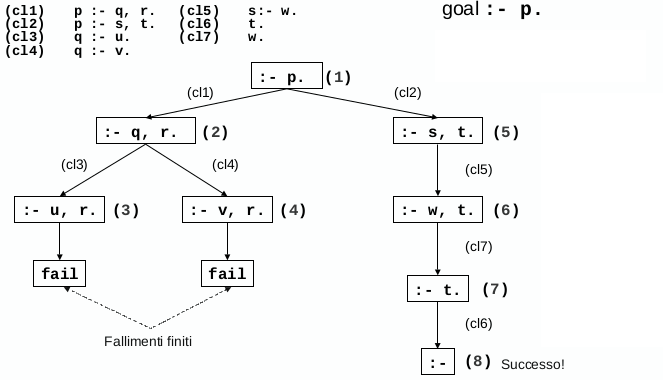
\includegraphics[scale=0.7]{img/alb.png}
\end{center}
\end{esempio}
Ad ogni ramo di un albero SLD corrisponde una derivazione
SLD e o gni ramo che termina con il nodo vuoto $:-$ rappresenta una derivazione SLD di successo. La regola di calcolo influisce sulla struttura dell'albero per quanto riguarda sia l'ampiezza sia la profondità tuttavia non influisce su correttezza e completezza; quindi, qualunque sia $R$, il numero di cammini di successo (se in numero finito) è lo stesso in tutti gli alberi SLD costruibili per $P\cup \{G_0\}$ e $R$ influenza solo il numero di cammini di fallimento (finiti ed infiniti).
\begin{esempio}
Ecco un altro esempio, con fallimento infinito, dove la clausola vuota può essere generata ma il Prolog non è in grado di trovare questa soluzione dato che la sua strategia di percorrimento dell’albero (implicito) di soluzioni è depth-first con backtracking :
\begin{center}
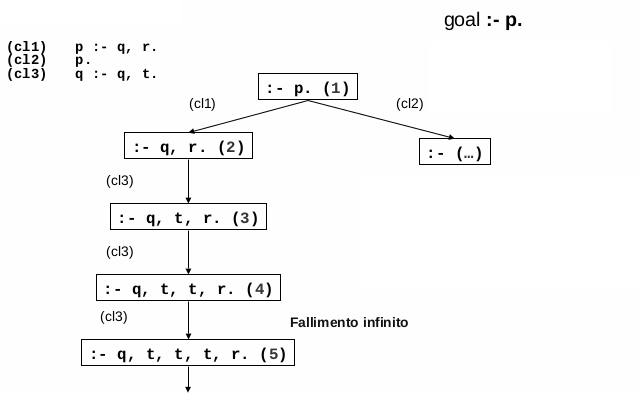
\includegraphics[scale=0.7]{img/alb2.png}
\end{center}
\end{esempio}
\begin{esempio}
%aggiungi esempio
\end{esempio}
\subsection{Cut e Backtracking}
Permette di controllare il backtracking, ovvero si tagliano certe possibilità di backtracking. Si indica con $!$ ed effettua un'interpretazione procedurale. \\
Come abbiamo intuito, le clausole nel data base di un programma
Prolog vengono considerate “da sinistra, verso destra” e “dall'alto al
basso”. Se un (sotto)goal fallisce, allora il dimostratore Prolog, sceglie un'alternativa, scandendo “dall'alto” verso “il basso” la lista delle clausole. Questo può essere controllato dal \textit{cut}. Un esempio:
\begin{minted}{prolog}
a :- b1, b2, ..., bk, !, ..., bn.
\end{minted}
Questo è l'effetto del cut:
\begin{itemize}
\item se il goal corrente \textit{G} unifica con \textit{a} e $b_1,...,b_k$ hanno successo, allora il dimostratore si impegna inderogabilmente alla scelta di C per dimostrare G
\item ogni clausola alternativa (successiva, in basso) per \textit{a} che unifica con \textit{G} viene ignorata
\item se un qualche $b_j$ con $j > k$ fallisse, il backtracking si fermerebbe al cut e le altre scelte sono rimosse dall'albero di derivazione
\item quando il backtracking raggiunge il cut, allora il cut fallisce e la ricerca procede dall’ultimo punto di scelta prima che \textit{G} scegliesse \textit{C}
\end{itemize}
%aggiungere gestione stack di prolog
vediamo un albero di derivazione in caso di cut:
\begin{center}
	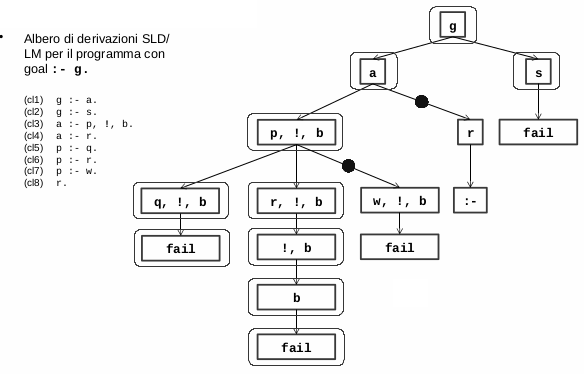
\includegraphics[scale=0.8]{img/cut.png}
\end{center}
Si hanno due tipi di cut:
\begin{itemize}
\item \textbf{green cut: } utili per esprimere “determinismo” (e quindi per rendere più efficiente il programma)
\item \textbf{red cut: } usati per soli scopi di efficienza, hanno per caratteristica principale quella di omettere alcune condizioni esplicite in un programma e, soprattutto, quella di modificare la semantica del programma equivalente senza cuts. Sono indesiderabili ma utili
\end{itemize}
consideriamo il seguente codice:
\begin{minted}{prolog}
/* merge di due liste ordinate*/

merge([X | Xs], [Y | Ys], [X | Zs]) :-
	X < Y,
	merge(Xs, [Y | Ys], Zs).
merge([X | Xs], [Y | Ys], [X, Y | Zs]) :-
	X = Y,
	merge(Xs, Ys, Zs).
merge([X | Xs], [Y | Ys], [Y | Zs]) :-
	X > Y,
	merge([X | Xs], Ys, Zs).
merge([], Ys, Ys).
merge(Xs, [], Xs).

/+ minimo tra due numeri */

minimum(X, Y, X) :- X =< Y.
minimum(X, Y, Y) :- Y < X.
\end{minted}
vediamo cosa succede:
\begin{center}
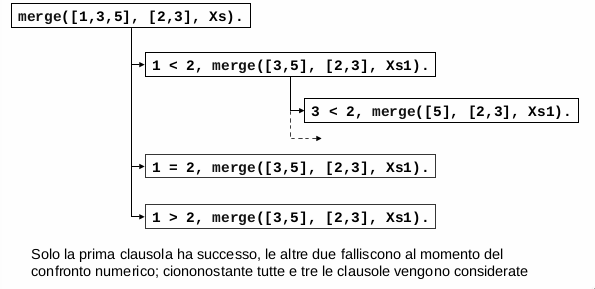
\includegraphics[scale=0.8]{img/cut2.png}
\end{center}
consideriamo la seguente query:
\begin{shaded}
\begin{lstlisting}[language=bash]
?- merge([], [], Xs).
Xs = [];
Xs = [];
False.
\end{lstlisting}
\end{shaded}
si ha una soluzione di troppo.\\
Un programma Prolog si dice \textbf{deterministico} quando una sola delle clausole serve (o si vorrebbe servisse) per provare un dato goal. Si usano quindi i green cuts:
\begin{minted}{prolog}
merge([X | Xs], [Y | Ys], [X | Zs]) :-
	X < Y, !,
	merge(Xs, [Y | Ys], Zs).
merge([X | Xs], [Y | Ys], [X, Y | Zs]) :-
	X = Y, !,
	merge(Xs, Ys, Zs).
merge([X | Xs], [Y | Ys], [Y | Zs]) :-
	X > Y, !,
	merge([X | Xs], Ys, Zs).
merge([], Ys, Ys) :- !.
merge(Xs, [], Xs) :- !.
\end{minted}
ottenendo:
\begin{shaded}
\begin{lstlisting}[language=bash]
?- merge([], [], Xs).
Xs = [];
False.
\end{lstlisting}
\end{shaded}
ovvero:
\begin{center}
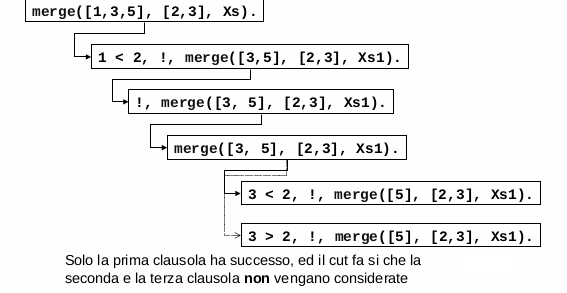
\includegraphics[scale=0.8]{img/cut3.png}
\end{center}
il programma del minimo diventa:
\begin{minted}{prolog}
minimum(X, Y, X) :- X =< Y, !.
minimum(X, Y, Y) :- Y < X, !.
\end{minted}
\textit{qui il secondo cut è ridondante ma viene messo per simmetria}.\\
Una volta che il programma ha fallito la prima clausola (ovvero il
test X =< Y) al sistema Prolog non rimane che controllare la
clausola seguente. Riscrivo in maniera non simmetrica:
\begin{minted}{prolog}
minimum(X, Y, X) :- X =< Y, !.
minimum(X, Y, Y).
\end{minted}
Qui si ha un red cut dato che taglia solo delle soluzioni, portando anche a risultati errati.\\
\subsection{Predicati Meta-Logici}
Vediamo il predicato:
\begin{minted}{prolog}
celsius_fahrenheit(C, F) :- C is 5/9 * (F - 32).
\end{minted}
Questo predicato non è invertibile. Si deve decidere qual è l'input e qual è l'output. Per questi problemi si hanno i \textit{predicati meta-logici}. La ragione di questo effetto (della non invertibilità) sta nell'uso che abbiamo fatto di vari predicati aritmetici nel corpo dei predicati (>, <, =<, is, etc), per poter usare i predicati aritmetici che usano direttamente l'hardware abbiamo sacrificato la semantica dei
nostri programmi.\\
I predicati meta-logici principali trattano le variabili come oggetti del linguaggio e ci permettono di riscrivere molti programmi che usano i predicati aritmetici di sistema come predicati dalla semantica “corretta” ed dal comportamento invertibile. Si hanno due predicati importanti:
\begin{itemize}
\item \textit{var(X):}  vero se \textit{X} è una variabile logica
\item \textit{nonvar(X):}  vero se \textit{X} non è una variabile logica
\end{itemize}
ovvero:

\begin{shaded}
\begin{lstlisting}[language=bash]
?- var(foo).
No
?- var(X).
Yes
?- nonvar(42).
Yes
\end{lstlisting}
\end{shaded}

il nostro programma dei gradi diventa:
\begin{minted}{prolog}
celsius_fahrenheit(C, F) :- 
  var(C), nonvar(F), C is 5/9 * (F - 32).
celsius_fahrenheit(C, F) :- 
  var(F), nonvar(C), F is (9/5 * C) + 32
\end{minted}
con var decido che clausola usare. L'uso di questi predicati ci permette di scrivere programmi efficienti e semanticamente corretti.
\subsection{Ispezione dei termini}
Posso chiedere a prolog se ho a che fare con termini atomici o scomposti, con i seguenti predicati:
\begin{itemize}
\item \textit{atomic(X): }vero se \textit{X} è un numero od una costante
\item \textit{compound(X):} vero se non \textit{atomic(X)}
\end{itemize}
Ho anche per manipolare un termine \textit{Term}:
\begin{itemize}
\item \textit{functor(Term, F, Arity)},
vero se \textit{Term} è un termine, con\textit{ Arity }argomenti, il cui funtore (simbolo di funzione o di predicato) è \textit{F}
\item \textit{arg(N, Term, Arg)},
vero se l’N-esimo argomento di \textit{Term }è \textit{Arg}
\item \textit{Term =.. L}
questo predicato, =..,viene chiamato (per motivi storici) \textit{univ}; è vero quando L è una lista il cui primo elemento è il funtore di \textit{Term} ed i rimanenti elementi sono i suoi argomenti
\end{itemize}
ovvero:
\begin{minted}{prolog}
?- functor(foo(24), foo, 1).
YES
?- functor(node(x, _, [], []), F, 4).
F = node
Yes
?- functor(Term, bar, 2).
Term = bar(_0,_1)
Yes
?- arg(3, node(x, _, [], []), X).
X = []
Yes
?- arg(1, father(X, lot), haran).
X = haran
Yes
?- father(haran, lot) =.. Ts.
Ts = [father, haran, lot]
Yes
?- father(X, lot) =.. [father, haran, lot].
X = haran
Yes
\end{minted}
\subsection{Programmazione di ordine superiore}
Quando si formula una domanda per il sistema Prolog, ci si
aspetta una risposta che è un'istanza (individuale) derivabile dalla knowledge base. Col backtracking ne abbiamo una alla folta, se le voglio tutte o voglio altri modi per acceder agli insiemi ho:
\begin{itemize}
\item \textit{findall(Template, Goal, Set):} 
\begin{itemize}
\item Vero se Set contiene tutte le istanze di Template che soddisfano Goal
\item \textit{Le istanze di Template vengono ottenute mediante backtracking}
\end{itemize}
\item \textit{bagof(Template, Goal, Bag):}
\begin{itemize}
\item Vero se Bag contiene tutte le alternative di Template che soddisfano Goal
\item Le alternative vengono costruite facendo backtracking solo se vi sono delle variabili libere in Goal che non appaiono in Template
\item È possibile dichiarare quali variabili non vanno considerate libere al fine del backtracking grazie alla sintassi $Var^G$ come Goal; In questo caso Var viene pensata come una variabile esistenziale
\end{itemize}
\item \textit{setof(Template, Goal, Set)}, che si comporta come bagof, ma Set non contiene soluzioni duplicate
\end{itemize}
\newpage
ovvero:
\begin{shaded}
\begin{lstlisting}[language=bash]
/* findall */

?- findall(C, father(X, C), Kids).
C = _0
X = _1
Kids = [abraham, nachor, haran, isaac, lot, milcah, yiscah]
Yes.


/* bagof */

?- bagof(C, father(X, C), Kids).
C = _0
X = terach
KIDS = [abraham, haran, nachor];
C = _0
X = haran
KIDS = [lot, yiscah, milcah];
C = _0
X = abraham
KIDS = [isaac];
flase.

/* bagof con variabile esistenziale */

?- bagof(C, X^father(X, C), Kids).
C = _0
X = _1
Kids = [abraham, haran, lot, yiscah, nachor, isaac,...];
false.
\end{lstlisting}
\end{shaded}
\newpage
\subsection{Predicati di ordine superiore e meta variabili}
Buona parte di questi predicati funziona grazie al meccanismo
delle meta-variabili, ovvero variabili interpretabili come goals. Per esempio si ha il predicato \textit{call}:
\begin{minted}{prolog}
call(G) :- G.
\end{minted}
Possiamo quindi definire il predicato \textit{applica }che valuta una query composta da un funtore e da una lista di argomenti:
\begin{minted}{prolog}
applica(P, Argomenti) :-
  P =.. PL, append(PL, Argomenti, GL), Goal =.. GL, call(Goal).
\end{minted}
\begin{shaded}
\begin{lstlisting}[language=bash]
?- applica(father, [X, C]).
X = terach
C = abraham;
X = terach
C = nachor;
false

?- applica(father(terach), [C]).
C = abraham;
C = nachor;
false
\end{lstlisting}
\end{shaded}
\subsection{Manipolazine della base di Dati}
Un programma Prolog è costituito da una base di dati (o knowledge base) che contiene \textbf{fatti} e \textbf{regole}. Il Prolog però mette a disposizione anche altri predicati che servono a manipolare direttamente la base di dati. Ovviamente, questi predicati vanno usati con molta attenzione, dato che modificano dinamicamente lo stato del programma:
\begin{itemize}
\item \textit{listing}
\item \textit{assert, asserta, assertz}
\item \textit{retract}
\item \textit{abolish}
\end{itemize}
se si ha una knowledge base vuota si avrà:
\begin{shaded}
\begin{lstlisting}[language=bash]
?- listing.
Yes
\end{lstlisting}
\end{shaded}
ovvero solo yes e il \textit{listing} è vuoto. Aggiungo qualcosa alla base dati con:
\begin{shaded}
\begin{lstlisting}[language=bash]
?- assert(happy(maya)).
true
\end{lstlisting}
\end{shaded}
che risponderà sempre \textit{true}, ora si avrà:
\begin{shaded}
\begin{lstlisting}[language=bash]
?- listing.
happy(maya).
true
\end{lstlisting}
\end{shaded}
e la base dati non sarà più vuota. Aggiungo altro alla base dati:
\begin{shaded}
\begin{lstlisting}[language=bash]
?- assert(happy(vincent)).
true

?- assert(happy(marcellus)).
true

?- assert(happy(butch)).
true

?- assert(happy(vincent)).
true
\end{lstlisting}
\end{shaded}
il \textit{listing} ora darà:
\begin{shaded}
\begin{lstlisting}[language=bash]
?- listing.
happy(mia).
happy(vincent).
happy(marcellus).
happy(butch).
happy(vincent).
true
\end{lstlisting}
\end{shaded}
\textit{si nota come un dato si possa inserire più volte}.\\
si possono anche asserire regole usando \textit{assert} e mettendo la regola tra parentesi:
\begin{shaded}
\begin{lstlisting}[language=bash]
?- assert( (naive(X) :- happy(X)) ).
true

?- listing.
happy(mia).
happy(vincent).
happy(marcellus).
happy(butch).
happy(vincent).
naive(A) :-
happy(A).
true
\end{lstlisting}
\end{shaded}
possiamo anche rimuovere fatti e regole con \textit{retract}, riprendendo dagli esempi sopra:
\begin{shaded}
\begin{lstlisting}[language=bash]
?- retract(happy(marcellus)).
true

?- listing.
happy(mia).
happy(vincent).
happy(butch).
happy(vincent).
naive(A) :-
happy(A).
true
\end{lstlisting}
\end{shaded}
inoltre si ha che \textit{retract} rimuove solo la prima occorrenza:
\begin{shaded}
\begin{lstlisting}[language=bash]
?- listing.
happy(mia).
happy(vincent).
happy(butch).
happy(vincent).
naive(A) :-
happy(A).
true

?- retract(happy(vincent)).
true

?- listing.
happy(mia).
happy(butch).
happy(vincent).
naive(A) :-
happy(A).
true
\end{lstlisting}
\end{shaded}
Per rimuovere tutte le nostre asserzioni possiamo usare una variabile:
\begin{shaded}
\begin{lstlisting}[language=bash]
?- retract(happy(X)).
X = mia;
X = butch;
X = vincent;
false

?- listing.
naive(A) :-
happy(A)
true
\end{lstlisting}
\end{shaded}
Per avere più controllo su dove vengono aggiunti fatti e regole possiamo usare le due varianti di assert:
\begin{enumerate}
\item \textit{assertz:} inserisce l’asserzione alla fine della knowledge base
\item \textit{asserta:} inserisce l’asserzione all'inizio della knowledge base
\end{enumerate}
ovvero, partendo da una base dari vuota:
\begin{shaded}
\begin{lstlisting}[language=bash]
?- assert(p(b)), assertz(p(c)), asserta(p(a)).
true

?- listing.
p(a).
p(b).
p(c).
true
\end{lstlisting}
\end{shaded}
\textbf{manipolarei dati in prolog pè utile ma rischioso!}\\
La manipolazione dati può essere usata per memorizzare i risultati
intermedi di varie computazioni, in modo da non dover rifare
delle queries dispendiose in futuro: semplicemente si ricerca
direttamente il fatto appena asserito. Questa tecnica si chiama \textbf{memorization} o \textbf{caching}.
\begin{esempio}
Creiamo una tavola di addizioni manipolando la knowledge base:
\begin{minted}{prolog}
addition_table(A) :-
  member(B, A),
  member(C, A),
  D is B + C,
  assert(sum(B, C, D)),
  fail.
\end{minted}
dove \textit{member(X, Y)} controlla che il predicato X appartenga alla lista Y.\\
\begin{shaded}
\begin{lstlisting}[language=bash]
?- addition_table([0, 1, 2, 3, 4, 5, 6, 7, 8, 9]).
false
\end{lstlisting}
\end{shaded}
La risposta è false; ma non è la risposta che ci interessa, bensì
l’effetto (collaterale) che l’interrogazione ha sulla knowledge base:
\begin{shaded}
\begin{lstlisting}[language=bash]
?- listing(sum).
sum(0, 0, 0).
sum(0, 1, 1).
sum(0, 2, 2).
sum(0, 3, 3).
...
sum(9, 9, 18).
true
\end{lstlisting}
\end{shaded}
potremmo ora rimuovere tutti questi fatti non con il solito 
\begin{shaded}
\begin{lstlisting}[language=bash]
?- retract(sum(X, Y, Z)).
\end{lstlisting}
\end{shaded}
che dovremmo ripetere ogni volta per ogni fatto ma con:
\begin{shaded}
\begin{lstlisting}[language=bash]
?- retract(sum(_, _, _)), fail.
false
\end{lstlisting}
\end{shaded}
Ancora una volta, lo scopo del \textit{fail} è di forzare il backtracking. Il Prolog rimuove il primo fatto con funtore sum dalla base di dati e poi fallisce. Quindi fa bactrack e rimuove il fatto successivo e così via. Alla fine, dopo aver rimosso tutti i fatti con funtore sum, la query fallirà completamente ed il Prolog risponderà (correttamente) con un \textit{false}. Ma anche in questo caso a noi interessa unicamente l’effetto collaterale sulla knowledge base.
\end{esempio}
\subsection{Input e Output}
I predicati primitivi principali per la gestione dell'I/O sono
essenzialmente due, \textbf{read} e \textbf{write}, a cui si aggiungono i vari predicati per la gestione dei files e degli streams: \textbf{open, close, seek}, etc...
\textit{write} è l'equivalente del metodo \textit{toString} JAva su un oggetto di classe "termine" mentre \textit{read} invoca il parser prolog:
\begin{shaded}
\begin{lstlisting}[language=bash]
?- write(42).
42
true

?- foo(bar) = X, write(X).
foo(bar)
X = foo(bar)
?- read(What).
|: foo(42, Bar).
What = foo(42, _G270).

?- read(What), write('I just read: '), write(What).
|: read(What).
I just read: read(_G301)
What = read(_G301).

?- open(’some/file/here.txt’, write, Out),
write(Out, foo(bar)), put(Out, 0’.), nl(Out),
close(Out).
true % But file ”some/file/here.txt” now contains the term ’foo
(bar).’

?- open(’some/file/here.txt’, read, In),
read(In, What)
close(In).
What = foo(bar)
\end{lstlisting}
\end{shaded}
\textbf{open} e \textbf{close} servono per leggere e scrivere files; la versione più semplice di open ha con tre argomenti: un atomo che rappresenta il nome del file, una “modalità” con cui si apre il file ed un terzo argomento a cui si associa l’identificatore del file.\\
Esiste anche il predicato \textbf{put} che emette un carattere sullo stream ed il predicato nl che mette un ‘newline’ sullo stream.\\
Il Prolog usa la notazione \textit{0'c} per rappresentare i caratteri come termini
\subsection{Interpreti in Prolog}
Il Prolog si presta benissimo alla costruzione di interpreti per la manipolazione di linguaggi specializzati (Domain Specific Languages (DSLs)). Vediamo qualche esempio:
\begin{itemize}
\item intepreti per Automi (a Stati Finiti, a Pila, Macchine di Turing)
\item sistemi per la deduzione automatica
\item sistemi per la manipolazione del Linguaggio Naturale (Natural
Language Processing (NLP))
\end{itemize}
Vediamo un automa:
\begin{center}
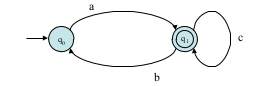
\includegraphics[scale=0.8]{img/aut.png}
\end{center}
i nodi rappresentano degli stati. Si ha uno stato inziale ($q_0$) e uno finale, denotato con un doppio cerchio, ($q_1$). Gli archi sono le transizioni tra due stati e nel nostro caso si generano caratteri. Nell'esempio ho solo stringhe che iniziano con $a$. In $q_1$ posso fermarmi e generare solo la stringa $a$ o produrre altri caratteri in numero variabile. Le stringhe qui prodotte saranno del tipo $ac^n(ba)^n$, con $n\geq 0$.\\
\newpage
Per decidere se una certa sequenza di simboli è riconosciuta dall’automa possiamo costruire il seguente predicato:
\begin{minted}{prolog}
/* definisco l'interprete */
accept([I | Is], S) :-
  delta(S, I, N),
  accept(Is, N).
accept([], Q) :- final(Q). /* è l'uscita, se ho una lista vuota
                               ho generato tutto */

/* richiesta di riconoscere un automa con stato iniziale S
    poi si usa l'accept con input che rappresenta la stringa
     considerando lo stato inziale S */
recognize(Input) :- initial(S), accept(Input, S).

initial(q0). % stato iniziale
final(q1). % stato finale

/* definisco le transizioni, con delta a tre argomenti */
delta(q0, a, q1).
delta(q1, b, q0).
delta(q1, c, q1).
\end{minted}
\begin{shaded}
\begin{lstlisting}[language=bash]
?- recognize([a, b, a, c, c, b, a]).
Yes

?- recognize([a, b, a, c, b]).
No
\end{lstlisting}
\end{shaded}
vediamo cosa succede:\\
prendo la lista $[a,\,b,\,a,\,c,\,c,\,b,\,a]$, si hanno le seguenti sostituzioni: $I\backslash a$ e $S\backslash q0$. Avrò quindi:
\begin{minted}{prolog}
delta(q0, a, N).
accept([b, ...], N).
\end{minted}
ora si hanno le seguenti sostituzoni: $N\backslash q1$:
\begin{minted}{prolog}
accept([b, ...], q1). % è il nuovo goal
\end{minted}
\newpage
unifico ancora con le sostituzioni $I2\backslash b$ e $Is\backslash [a,c,c,b,a]$:
\begin{minted}{prolog}
delta(q1, b, N2).
accept([a, c, c, b, a], N2).
\end{minted}
ad un certo punto arriveremo alla fine:
\begin{minted}{prolog}
accept([], q1).
\end{minted}
che unifica con la seconda clausola, sostituendo $q1\backslash Q$, arrivando a:
\begin{minted}{prolog}
final(q1).
\end{minted}
\subsection{Meta-interpreti}
Possiamo scrivere degli interpreti più complicati e/o specializzati
se accettiamo di rappresentare i programmi con una sintassi
leggermente diversa:
\begin{minted}{prolog}
rule(append([], X, X)).
rule(append([X | Xs], Ys, [X | Zs]), [append(Xs, Ys, Zs)]).

solve(Goal) :- solve(Goal, []). /* lista goal e lista di appoggio 
                                    dove mettere i goal restanti */

solve([], []). % clausola di uscita

solve([], [G | Goals]) :-
  solve(G, Goals).
solve([A | B], Goals) :-
  append(B, Goals, BGoals),
  solve(A, BGoals).
solve(A, Goals) :-
  rule(A),
  solve(Goals, []).
solve(A, Goals) :-
  rule(A, B),
  solve(B, Goals).
\end{minted}
Il programma \textit{solve} è un meta-interprete per i predicati \textit{rule }che compongono il nostro sistema (o programma).\\
\newpage
Si può avere incertezza nella conoscenza espressa. Si può avere unsa sorta di statistica:
\begin{minted}{prolog}
solve_cf(true, 1) :- !.
solve_cf((A, B), C) :-
  !,
  solve_cf(A, CA),
  solve_cf(B, CB),
  minimum(CA, CB, C).
solve_cf(A, 1) :-
  builtin(A),
  !,
  call(A).
solve_cf(A, C) :-
  rule_cf(A, B, CR),
  solve_cf(B, CB),
  C is CR * CB.
\end{minted}
Il programma \textit{solve}$\_$\textit{cf} è un meta-interprete per stabilire se un goal G è vero e quanto siamo certi che sia vero.
\chapter{Lisp}
Usa il paradigma funzionale. I programmi computano combinando “valori” (rappresentati in memoria) trasformati da chiamate a funzioni. Si ha che i programmi sono funzioni matematiche, funzioni primitive o composte. Si ha il concetto matematico della \textbf{trasparenza referenziale} ovvero:
\begin{center}
\textit{il significato del tutto si può determinare dal significato delle parti}
\end{center}
questo concetto rende possibile la composizione di funzioni.\\
Ogni funzione denota un valore ottenuto tramite una mappa a
partire dagli "argomenti". Nel paradigma funzionale vi sono oggetti di vario tipo e strutture di controllo, ma vengono raggruppati logicamente in modo
diverso da come invece accade nel paradigma imperativo. In
particolare è utile pensare in termini di:
\begin{itemize}
\item espressioni (funzioni primitive e non)
\item modi di combinare tali espressioni per ottenerne di più
complesse (composizione)
\item modi e metodi di costruzione di “astrazioni” per poter far
riferimento a gruppi di espressioni per “nome” e per trattarle
come unità separate
\item operatori speciali (condizionali ed altri ancora, che verranno
introdotti in seguito)
\end{itemize}
ricordiamo che una funzione è una regola per associare gli elementi di un insieme (\textbf{dominio}) a quelli di un altro insieme (\textbf{codominio}). In un linguaggio funzionale l'argomento della funzione è mappato in particolari locazioni di memoria e non può essere modificato. Le composizioni di funzioni sono spesso organizzate in maniera ricorsiva. Le funzioni sono oggetti di prima classe e possono essere puntatori a una funzione, una struttura dati e possono essere costruite durante l’esecuzione di un programma e ritornate come valore di un’altra funzione. Ilinguaggi funzionali consentono l’uso di funzioni di ordine superiore, cioè funzioni che prendono altre funzioni come argomenti e che possono restituirne come valore, in modo assolutamente generale. Nei linguaggi funzionali puri non esistono strutture di controllo iterative come while e for; questi sostituiti da ricorsione combinata con gli operatori speciali condizionali.\\
\textbf{Lisp} è una famiglia di linguaggi con due dialetti principali: \textbf{Common Lisp} e \textbf{Scheme}. Lo studio del LISP in una delle sue incarnazioni è importante dato che il linguaggio è uno dei più vecchi rappresentanti del paradigma di programmazione funzionale. Le versioni minimali di Lisp ammettono:
\begin{itemize}
\item funzioni primitive su \textbf{liste}
\item un'operatore speciale \textbf{lambda} per creare funzioni
\item un'operatore codizionale \textbf{cond}
\item un piccolo insieme di predicati ed operatori speciali
\end{itemize}
Una prima cosa da notare è che in LISP ogni “espressione” denota un
“valore”.
\begin{shaded}
\begin{lstlisting}[language=bash]
prompt> 42
42

prompt> ”Sapete che cos’e` ’42’?”
”Sapete che cos’e` ’42’?”
\end{lstlisting}
\end{shaded} Si ha la seguente notazione:
$$/f\,\,\, x_1\,\,\,...\,\,\, x_n)$$
Le parentesi iniziali e finale sono obbligatorie (vedremo più in là
che ciò ha conseguenze importanti) e gli spazi (almeno uno)
sono necessari per separare tra di loro la funzione e gli argomenti.
le operazioni matematiche elementari sono funzioni:
\begin{shaded}
\begin{lstlisting}[language=bash]
prompt> (+ 40 2)
42

prompt> (- 84 42)
42

prompt> (* 2 3 7)
42
\end{lstlisting}
\end{shaded}
si possono avere più argomenti:
\begin{shaded}
\begin{lstlisting}[language=bash]
prompt> (+ 2 10 10 20)
42
\end{lstlisting}
\end{shaded}
e per le composte si ha che al posto di un valore posso avere la chiamata ad una funzione: 
\begin{shaded}
\begin{lstlisting}[language=bash]
prompt> (+ 2 (* 2 10) 20)
42

prompt> (+ (* 3 (+ (* 2 4) (+ 3 2))) (+ (- 10 8) 1))
42
\end{lstlisting}
\end{shaded}
solitamente si allinea con gli argomenti (ovvero gli \textbf{operandi}) di una chiamata allineati verticalmente:
\begin{shaded}
\begin{lstlisting}[language=bash]
prompt> (+ (* 3
              (+ (* 2 4)
                 (+ 3 2)))
           (+ (- 10 8)
              1))
42
\end{lstlisting}
\end{shaded}
Notiamo come le funzioni aritmetiche elementari + e * in (Common) LISP
rispettano i vincoli di “campo” algebrico:
\begin{shaded}
\begin{lstlisting}[language=bash]
prompt> (+)
0

prompt> (*)
1
\end{lstlisting}
\end{shaded}
Le funzioni aritmetiche elementari - e / in (Common) LISP richiedono almeno
un argomento e rappresentano in questo caso il “reciproco”, sempre in senso
algebrico:
\begin{shaded}
\begin{lstlisting}[language=bash]
prompt> (- 42)
-42

prompt> (/ 42)
1/42
\end{lstlisting}
\end{shaded}
posso avere:
\begin{itemize}
\item numeri interi, numeri in virgola mobile (es. $3.5$ o $6.02E+21$), numeri razionali (es. $-3/42$) o numeri complessi ($\#C (0 1)$)
\item booleani $T$ e $NIL$
\item stringhe (es $"sono\,\,\, una \,\,\,stringa"$)
\item operatiori sui booleani $null,\,\,\,and,\,\,\, or,\,\,\,not$
\item funzioni sui numeri \textit{+ - / * mod sin cos sqrt tan atan plusp > <= zerop}
\end{itemize}
la valutazione delle funzioni va da sinistra a destra e produce i valori $v_1\,\,\,...\,\,\, v_n$ a cui successivamente verrà applicata la funzione in maniera \textit{inerentemente ricorsiva}. Questa valutazione non è seguita da alcuni operatori come \textit{if, cond, defun, defparameter, quote, etc...}.\\
Le variabili si definiscono con \textit{defparameter}:
\begin{shaded}
\begin{lstlisting}[language=bash]
prompt> (defparameter quarantadue 42)
quarantadue
\end{lstlisting}
\end{shaded}
ora il simbolo quarantadue ha ora associato il valore 42.\\
Le funzioni si possono definire usando l’operatore speciale defun (nome (argomenti) (corpo funzione)):
\begin{shaded}
\begin{lstlisting}[language=bash]
prompt> (defun quadrato (x) (* x x))
quadrato
\end{lstlisting}
\end{shaded}
L'operatore defun associa il corpo della funzione al nome
nell’ambiente globale del sistema Common Lisp e restituisce come valore il nome della funzione. Una volta definita, una funzione viene eseguita (o chiamata) usando la regola descritta precedentemente:
\begin{shaded}
\begin{lstlisting}[language=bash]
prompt> (quadrato quarantadue)
1764

prompt> (- (quadrato (+ 20 22)) 10)
1754

prompt> (defun somma-di-quadrati (x y)
           (+ (quadrato x) (quadrato y)))
somma-di-quadrati

prompt> (- (somma-di-quadrati 6 3) 3)
42
\end{lstlisting}
\end{shaded}
i nomi delle funzioni possono contenere il carattere "-" in quanto non si cra ambiguità con la funzione "-(...)", questo succede anche con \textit{(, ), \#, ‘, ’, ”} e con la virgola.\\
Per valutare le funzioni si ha la costruzione di un \textbf{activation frame}, i parametri formali di una funzione vengono associati ai valori (si passa tutto per valore senza effetti collaterali). Il corpo della funzione viene valutato (ricorsivamente) tenendo conto di questi legami in maniera statica, bisogna tener presente cosa accade con variabili che risultano
“libere” in una sotto-espressione. Ad ogni sotto-espressione del corpo si sostituisce il valore che essa denota (computa). l valore (valori) restituito dalla funzione è il valore del corpo della funzione (che non è altro che una sotto-espressione), Quando il valore finale viene ritornato i legami temporanei ai parametri formali spariscono (lo stack di sistema subisce una “pop” l’activation frame viene rimosso). Per esempio:
\begin{shaded}
\begin{lstlisting}[language=bash]
prompt> (defun doppio (n) (* 2 n))
doppio

prompt> (doppio 3)
6
\end{lstlisting}
\end{shaded}
\begin{itemize}
\item estende l’ambiente globale con il legame tra doppio e la sua definizione
\item estende l’ambiente globale con quello locale che contiene i legami tra
parametri formali e valori dei parametri attuali, un activation frame viene inserito in cima allo stack di valutazione
\item valuta il corpo della funzione
\item ripristina l’ambiente di partenza, l’activation frame viene rimosso dalla cima dello stack di valutazione
\end{itemize}

 Per la valutazione di una funzione F, l’ambiente deve eseguire i seguenti sei passi:
\begin{enumerate}
\item mettere i parametri in un posto dove la procedura possa recuperarli
\item trasferire il controllo alla procedura
\item allocare le risorse (di memorizzazione dei dati) necessarie alla procedura
\item effettuare la computazione della procedura
\item mettere i risultati in un posto accessibile al chiamante
\item restituire il controllo al chiamante
\end{enumerate}

Queste operazioni agiscono sui registri a disposizione e sullo “stack” utilizzato dal runtime (esecutore) del linguaggio.\\Lo spazio richiesto per salvare (sullo stack) tutte le informazioni necessarie all’esecuzione di
una funzione F ed al ripristino dello stato precedente alla chiamata è quindi costituito da:
\begin{itemize}
\item Spazio per i registri da salvare prima della chiamata di una sotto funzione
\item Spazio per l’indirizzo di ritorno (nel codice del corpo della funzione)
\item Spazio per le variabili, definizioni locali, e valori di ritorno
\item Spazio per i valori degli argomenti
\item Spazio per il riferimento statico (static link)
\item Spazio per il riferimento dinamico (dynamic link)
\item Altro spazio dipendente dal particolare linguaggio e/o politiche di allocazione del compilatore
\end{itemize}
% aggiungere disegni
La gestione dello static link in Common Lisp è in realtà più complicato,
dato che il linguaggio ammette la creazione a runtime di funzioni che si
devono ricordare il valore delle loro variabili libere al momento della
loro creazione. Queste funzioni sono implementate con particolari strutture dati chiamate \textbf{chiusure (closures)}, che chiudiono i valori delle loro variabili libere. Si possono quindi creare funzioni anonime, le \textbf{lambda}:
\begin{center}
$$(lambda\,\,(x_1\,\,...\,\,x_n)\,\,<e>)$$
\end{center}
con $<e>$ espressione detta \textbf{lambda-expression}:
\begin{shaded}
\begin{lstlisting}[language=bash]
(lambda (x) (+ 2 x))

((lambda (x) (+ 2 x)) 40)
42
\end{lstlisting}
\end{shaded}
pensiamo ora alla creazione come quella per il valore assoluto che presenta più casistiche. Useremo il costrutto \textbf{cond}:
$$(cond\,\,(c_1\,\,e_1),\,\,...\,\,(c_n\,\,e_n))$$
ovvero:
\begin{minted}{lisp}
(defun valore-assoluto (x)
   (cond ((> x 0) x)
         ((= x 0) 0)
         ((< x 0) (- x))))
\end{minted}
l'operatore cond verifica ogni coppia di espressioni e se il risultato è T ritorna il valore della seconda espressione altrimenti passa lal coppia successiva. Se non ci sono più coppie valutabili restituisce NIL
\begin{shaded}
\begin{lstlisting}[language=bash]
prompt> (valore-assoluto 3)
3

prompt> (valore-assoluto -42)
42
\end{lstlisting}
\end{shaded}
potevo anche definirlo come:
\begin{minted}{lisp}
(defun valore-assoluto (x)
    (cond ((> x 0) x)
          (T (- x))))
\end{minted}
e anche con:
\begin{minted}{lisp}
(defun valore-assoluto (x)
   (if (> x 0) x (- x)))
\end{minted}
si hanno ovviamente anche gli operatori booleani \textit{and, or e not}:
\begin{shaded}
\begin{lstlisting}[language=bash]
prompt> (and (> 42 0) (< -42 0))
T

prompt> (not (> 42 0))
NIL

prompt> (and)
T

prompt> (or)
NIL
\end{lstlisting}
\end{shaded}
ecco una funzione per approssimare la radice quadrata di un numero:
\begin{minted}{lisp}
(defun radice-quadrata (x)
    (ciclo-radice-quadrata x 1.0))

(defun va-bene? (x c)
    (< (valore-assoluto (- x (quadrato c)))
       0.001))
       
(defun media (x y) (/ (+ x y) 2.0))

(defun migliora (c x) (media c (/ x c)))

(defun ciclo-radice-quadrata (x c)
    (if (va-bene? x c)
        c
        (ciclo-radice-quadrata x (migliora c x))))

\end{minted}
che esegue la seguente approssimazione:
$$1\to \frac{2}{1}=2 \to ((2+1)/2)=1,5$$
$$1,5 \to \frac{2}{1,5}=1,3333\to ((1,3333+1,5)/2)=1,4167$$
$$\cdots$$
con un errore massimo di 0,001. La prima congettura è per il numero 1.\\
Vediamo una funzione ricoriva come il fattoriale:
\begin{minted}{lisp}
(defun fattoriale (n)
    (if (= n 0)
        1
        (* n (fattoriale (- n 1)))))
\end{minted}
Questa funzione calcola il fattoriale di un numero utilizzando
una sequenza di valori intermedi che devono essere salvati da
qualche parte (ovvero sullo “stack” di attivazione di ogni
chiamata ricorsiva). \\
Vediamo anche Fibonacci:
\begin{minted}{lisp}
(defun fib (n)
     (cond ((= n 0) 1)
           ((= n 1) 1)
           (T (+ (fib (- n 2)) (fib (- n 1))))
            ))
\end{minted}
possiamo anche scrivere il fattoriale in una forma simile:
\begin{minted}{lisp}
(defun fatt-ciclo (n acc)
      (if (= n 0)
          acc
          (fatt-ciclo (- n 1) (* n acc))))
(defun fattoriale (n)
    (fatt-ciclo n 1))
\end{minted}
ovvero utilizzando uno degli argomenti come accumulatore. Con \textit{fatt-ciclo} si ha un "ciclo in incognito" che è d'aiuto al compilatore che può effettuare una funzione di jump. Una funzione così è detta \textbf{tail-ricorsive}.\\
Un insieme di funzioni mutualmente ricorsive può rappresentare una
macchina di Turing quindi, i linguaggi funzionali puri (senza assegnamenti e “salti”) sono Turing-completi.\\
Creaiamo ora una libreria per fare conti coi razionali. Innanzitutto assumiamo di aver a disposizione una funzione che
costruisce una rappresentazione di un numero razionale:
\begin{minted}{lisp}
(crea-razionale n d) Þ <il razionale n/d>
\end{minted}
Assumiamo anche di avere due funzioni numer and denom che
estraggono rispettivamente il numeratore n ed il denominatore d dalla
rappresentazione di un numero razionale <razionale n/d>:
\begin{minted}{lisp}
(defun somma-raz (r1 r2)
    (crea-razionale (+ (* (numer r1) (denom r2))
                       (* (numer r2) (denom r1)))
                    (* (denom r1) (denom r2))))
(defun molt-raz (r1 r2)
    (crea-razionale (* (numer r1) (numer r2))
                    (* (denom r1) (denom r2)))
(defun =-raz (r1 r2)
    (= (* (numer r1) (denom r2))
       (* (numer r2) (denom r1))))
       
...
\end{minted}
Una delle strutture più importanti del Lisp è la \textbf{Cons-Cell}, iovvero una coppia di puntatori a due elementi, \textit{car e cdr}:
\begin{minted}{lisp}
cons : <oggetto Lisp> x ́<oggetto Lisp> -> <cons-cell>
\end{minted}
\begin{shaded}
\begin{lstlisting}[language=bash]
prompt> (defparameter c (cons 40 2))
c

prompt> (car c)
40

prompt> (cdr c)
2
\end{lstlisting}
\end{shaded}
con questo costrutto si semplifica la libreria per i razionali:
\begin{minted}{lisp}
(defun crea-razionale (n d)
   (cons n d))

(defun numer (r) (car r))

(defun denom (r) (cdr r))
\end{minted}
\begin{shaded}
\begin{lstlisting}[language=bash]
prompt> (denom (crea-razionale 42 7))
7
\end{lstlisting}
\end{shaded}
La funzione cons genera in memoria dei grafi di puntatori
arbitrariamente complessi. Questi grafi vengono rappresentati in una tradizionale notazione detta \textit{box-and-pointer}:
\begin{center}
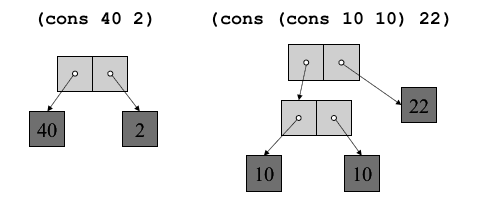
\includegraphics[scale=0.7]{img/cons.png}
\end{center}
Posso inserire anche T e NIL (rappresentato da una sbarra:
\begin{center}
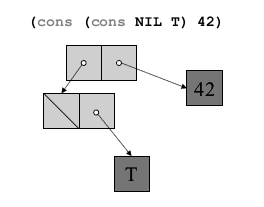
\includegraphics[scale=0.7]{img/cons2.png}
\end{center}
bediamo qualche esempio:
\begin{shaded}
\begin{lstlisting}[language=bash]
prompt> (cons NIL T)
(NIL . T) ; Notazione “dotted-pair”
          ; (“coppia-puntata”). Gli spazi
          ; sono significativi.
          
prompt> (cons 4 2)
(4 . 2)

prompt> (cons
\end{lstlisting}
\end{shaded}
La notazione “dotted pair” è l’unica “irregolarità sintattica infissa” in Lisp.		
\\
Quando si parla di liste in Lisp ci si riferisce a particolari configurazioni di cons-cells dove l’ultimo puntatore è NIL; la costante NIL è equivalente alla lista vuota ():
\begin{center}
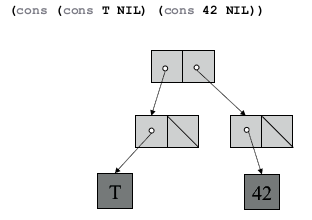
\includegraphics[scale=0.7]{img/cons3.png}
\end{center}
Una lista Lisp corrispondente a questa configurazione di cons-cells viene rappresentata tipograficamente come \textit{((T) 42)} che è uquivalente a \textit{((T . NIL) . (42 . NIL))}. Quindi una cons-cell con NIL come secondo
elemento (ovvero come cdr) viene stampata senza il punto ed il NIL:
\begin{shaded}
\begin{lstlisting}[language=bash]
prompt> (cons 42 nil)
(42)

prompt> (cons ”foo bar” nil)
(”foo bar”)
\end{lstlisting}
\end{shaded}
inoltre una cons-cell con una cons-cell come secondo elemento è stampata in modo “abbreviato”:
\begin{shaded}
\begin{lstlisting}[language=bash]
prompt> (cons 42 (cons 123 666))
(42 123 . 666)  ; Equivalente a (42 . (123 . 666))

prompt> (cons 42 (cons ”foo bar” nil))
(42 ”foo bar”)
;;; To`, una ’lista’.
\end{lstlisting}
\end{shaded}
cons si può usare anche per rappresentare una lista di oggetti:
\begin{minted}{lisp}
(defparameter L (cons 1 (cons 2 (cons 3 (cons 4 NIL)))))
\end{minted}
\begin{shaded}
\begin{lstlisting}[language=bash]
prompt> (car (cdr (cdr L)))
3
\end{lstlisting}
\end{shaded}

\begin{minted}{lisp}
(defparameter L (list 1 2 3 4))
\end{minted}
\begin{shaded}
\begin{lstlisting}[language=bash]
prompt> (car (cdr (cdr L)))
3
\end{lstlisting}
\end{shaded}
inoltre si ha la funzione list con un numero variabile di elementi:
\begin{shaded}
\begin{lstlisting}[language=bash]
prompt> (list -1 0 1 2 3)
(-1 0 1 2 3)
\end{lstlisting}
\end{shaded}
vediamo qualche manipolazione di una lista.\\
estraiamo l'n-esimo elemento:
\begin{minted}{lisp}
(defun list-ref (n list)
    (if (<= n 0)
        (car list)
        (list-ref (- n 1) (cdr list)))
\end{minted}
calocliamo la lunghezza di una lista:
\begin{minted}{lisp}
(defun lunghezza (l)
    (if (null l)
        0
        (+ 1 (lunghezza (cdr l)))))
\end{minted}
Si ha la funzione \textbf{nth}. Inoltre funzione cdr ritorna di fatto il “resto” di una lista e lo standard
Common Lisp fornisce anche l’ovvio sinonimo: rest e la funzione car ritorna il “primo” elemento di una lista; lo standard
Common Lisp fornisce anche il sinonimo first.\\
per fare l'append:
\begin{minted}{lisp}
(defun appendi (l1 l2)
    (if (null l1)
        l2
        (cons (car l1) (appendi (cdr l1) l2))))
\end{minted}
La funzione è ricorsiva e presenta una tipica forma di ricorsione “strutturale” sul resto di una lista (detta anche “cdr recursion” o “rest-recursion”).\\
In LISP si possono manipolare dati simbolici, costruendo liste come:
\begin{verbatim}
(a b c d e f g h I)
((gino 10) (ugo 10) (maria 2) (ettore 20))
\end{verbatim}
o anche:
\begin{minted}{lisp}
(+ quaranta 2)
(defun media (x y) (/ (+ x y) 2.0))
\end{minted}
Si ha l'operatore \textit{quote} che dice al LISP di non procedere alla valutazione di una (sotto)espressione:
\begin{minted}{lisp}
(quote <e>)
\end{minted}
con <e> che viene ritornato letteralmente
\begin{shaded}
\begin{lstlisting}[language=bash]
prompt> (quote 42)
42

prompt> (quote A)
A

prompt> (quote (1 B 3))
(1 B 3)

prompt> (quote (1 2 (3 4) (5 6 ”foo”)))
(1 2 (3 4) (5 6 ”foo”))
\end{lstlisting}
\end{shaded}
il quote ha anche una forma abbreviata: '<e>:
\begin{shaded}
\begin{lstlisting}[language=bash]
prompt> ’42 
42

prompt> ’A
A

prompt> ’(1 B 3)
(1 B 3)

prompt> ’(1 2 (3 4) (5 6 ”foo”))
(1 2 (3 4) (5 6 ”foo”))
\end{lstlisting}
\end{shaded}
il quote non agisce su numeri e stringhe che sono autovalutanti, ovvero essi sono
espressioni il cui valore ha la stessa rappresentazione tipografica dell'espressione
tipografica che li denota. I simboli (o identificatori) denotano invece I valori che sono loro associati (ad
esempio tramite defparameter). Inoltre le liste, se non quotate, rappresentano invece delle espressioni da valutare, ergo la
necessità di avere l’operatore di quote:
\begin{shaded}
\begin{lstlisting}[language=bash]
prompt> 42
42

prompt> ’42
42

prompt> ’”io sono una stringa”
”io sono una stringa”

prompt> ”io sono una stringa”
”io sono una stringa”

prompt> (list ’A ’B)
(A B)

prompt> ’(A B)
(A B)

prompt> ’(defun media (x y) (/ (+ x y) 2.0))
(DEFUN MEDIA (X Y) (/ (+ X Y) 2.0))

prompt> (defun media (x y) (/ (+ x y) 2.0))
MEDIA

prompt> (defparameter m
’(defun media (x y) (/ (+ x y) 2.0))
M

prompt> (third m) ; (car (cdr (cdr m)))
(X Y)
\end{lstlisting}
\end{shaded} 
e quindi si ha che \textbf{in LISP i programmi e i dati sono esattamente la stessa cosa}\\
In LISP si ha una ripartizione degli oggetti in due categorie:
\begin{itemize}
\item \textbf{atomi:} che sono simboli e numeri (ma non solo; ad esempio le stringhe):
\begin{shaded}
\begin{lstlisting}[language=bash]
prompt> (atom 3)
T
prompt> (atom ’un-simbolo)
T
prompt> (atom ”una stringa”)
T
prompt> (atom (cons -42 42))
NIL
prompt> (atom (list 1 2 3))
NIL
\end{lstlisting}
\end{shaded}
\item \textbf{cons-cell:} ovvero le liste
\end{itemize}
cons-cell più numeri, simboli, stringhe etc... costituiscono le \textbf{Symbolic Expression (sexp's)}\\
Dato che programmi e sexp’s in Lisp sono equivalenti, possiamo dare le seguenti regole di valutazione (ed implementarle nella funzione \textit{eval}). data un sexp's:
\begin{itemize}
\item se è un atomo:
\begin{itemize}
\item se è un numero ritorna il valore
\item se è una stringa ritornala così com'è
\item se è un simbolo ne estrae il valore dall'ambiente corrente e ne restituisce il valore, se non ha un valore associato da errore
\end{itemize}
\item se è una cons-cell si ha:
\begin{itemize}
\item Se O è un operatore speciale, allora la lista $(0\, A_1\,...\,A_n)$ viene valutata in modo speciale
\item Se O è un simbolo che denota una funzione nell'ambiente corrente, allora questa
funzione viene applicata \textit{apply} alla lista $(VA_1\,...\, VA_n)$ che raccoglie i
valori delle valutazioni delle espressioni $A_1\,...\,A_n$
\item Se O è una Lambda Expression la si applica alla lista che $(VA_1\,...\, VA_n)$
che raccoglie i valori delle valutazioni delle espressioni $A_1\,...\,A_n$
\item altrimenti segnala errore
\end{itemize}
\end{itemize}
\newpage
definisco il fattoriale:
\begin{minted}{lisp}
(defun fatt (n)
    (if (zerop n) 1 (* n (fatt (- n 1)))))
\end{minted}
\begin{shaded}
\begin{lstlisting}[language=bash]
prompt> (fatt 3)
n diventa associato a 3 (“bound to” 3):
(eval ‘(fatt 3))
-> (eval ‘(if (zerop 3) 1 (* 3 (fatt (- 3 1)))))
     ... -> (eval ‘(* 3 (fatt 2))))
         ... -> (eval ‘(*3 (* 2 (fatt 1))))
         ... -> (* 3 (* 2 (* 1 (fatt 0))))
     ... -> (* 3 (* 2 (* 1 1)))
... -> ... 6
\end{lstlisting}
\end{shaded}
eval applica la funzione al suo argomento, definendo i legami di N “in cascata” e
costruendo una espressione che alla fine verrà valutata, a partire dalla sotto-espressione
più annidata.\\ Questa struttura delle liste si presta bene alla ricorsione. \\
Vediamo la lunghezza di una lista:
\begin{minted}{lisp}
(defun lung (l)
   (if (null l)
       0
       (+ 1 (lung (rest l)))))
\end{minted}
\textit{last} restituisce l'ultimo elemento di una lista:
\begin{minted}{lisp}
(defun last-l (l)
    (cond ((null l) nil)
          ((atom l) ; Notare questo caso.
           (error ”L’argomento non e` una lista”))
          ((null (rest l)) (first l))
          (t (last-l (rest l))))
\end{minted}
si ha la ricorsione semplice, \textbf{ricorsione cdr} che è definita sul resto di una lista.\\
Vediamo come contare gli atomi di una sexp.\\
al caso base si ha che NIL, "()" conta 0, un atomo conta 1. l'ipotesi ricorsiva effettua il conta sul rest della lista e il caso passo analizza il first della lista e chiama la ricorsione.
\\
Esiste anche la ricorsione \textbf{car-cdr} che effettua la ricorsione sul car:
\begin{minted}{lisp}
(defun count-atoms(x) ; ‘x’ e` una sexp.
  (cond ((null x) 0)
        ((atom x) 1)
        (T (+ (count-atoms (first x))
              (count-atoms (rest x))))))
\end{minted}
Si definisce \textbf{profondità massima di annidamento} di una sexp come il numero di parentesi sospese (max è definito in Common Lisp:
\begin{minted}{lisp}
(defun prof (x)
   (cond ((null x) 1)
         ((atom x) 0)
         (t (max (+ 1 (prof (first x)))
                 (prof (rest x))))))
\end{minted}
vediamo la funzione flatten per appiattire una lista:
\begin{minted}{lisp}
(defun flatten (x) ; x e` s-espressione
    (cond ((null x) x) ; NB: (atom nil) = T
          ((atom x) (list x)) ; serve per usare
                    ; append
          (T (append (flatten (first x))
                     (flatten (rest x))))))
\end{minted}
\begin{shaded}
\begin{lstlisting}[language=bash]
prompt> (flatten ‘((((a (b (c d)) e) f)) 
(a b c d e f)

prompt> (flatten ‘a) 
(a)
\end{lstlisting}
\end{shaded}
per ottenere un'immagine speculare di una sexp:
\begin{minted}{lisp}
(defun mirror (x) ; x e` una sexp
    (if (atom x)
        x
    (append (mirror (rest x))
            (list (mirror (first x)))))))
\end{minted}
\begin{shaded}
\begin{lstlisting}[language=bash]
prompt> (flatten ‘((((a (b (c d)) e) f)) 
(f (e ((d c) b) a)
\end{lstlisting}
\end{shaded}
la funzione per invertire:
\begin{minted}{lisp}
(defun inverti (x)
    (cond ((null x) x)
          ((atom x) x) ; anche Sexp...
          (T (cons-end (first x)
                       (inverti (rest x))))))
\end{minted}
funzione circulate:
\begin{minted}{lisp}
(defun circulate (lst direction)
    (cond ((atom lst) lst)
          ((null lst) nil)
          ((eq direction 'left)
           (append (cdr lst) (list (car lst))))
          ((eq direction 'right)
           (cons (last-l lst) (but-last lst)))
          (T lst) ))
\end{minted}
\begin{shaded}
\begin{lstlisting}[language=bash]
prompt> (circulate '(1 2 3 4) 'left)
(2 3 4 1)

prompt> (circulate '(1 2 3 4) 'right)
(4 1 2 3)
\end{lstlisting}
\end{shaded}
Un problema preliminare che si pone in Lisp è quello di
controllare se due oggetti sono uguali; il Common Lisp mette a disposizione una pletora di predicati di uguaglianza con
semantica diversa. Si hanno due soluzioni principali:
\begin{itemize}
\item \textbf{eql:} viene usato per controllare l’uguaglianza di simboli, numeri interi e puntatori:
\begin{shaded}
\begin{lstlisting}[language=bash]
prompt> (eql 42 42)
T

prompt> (eql 42 3)
NIL

prompt> (eql ’quarantadue ’quarantadue)
T

prompt> (eql ’quarantadue quarantadue)
NIL

prompt> (eql ’quarantadue ’fattoriale)
NIL

prompt> (eql ’(42) ’(42))
NIL
\end{lstlisting}
\end{shaded}
\item \textbf{equal:} si comporta come \textit{eql}, ma è in grado di controllare se due liste sono uguali; in pratica non fa altro che applicare \textit{eql} ricorsivamente a tutti
gli atomi di una lista: se un'applicazione di \textit{eql} ritorna il valore NIL allora \textit{equal} fa lo stesso, altrimenti viene ritornato il valore T:
\begin{shaded}
\begin{lstlisting}[language=bash]
prompt> (equal 42 42)
T

prompt> (equal 42 3)
NIL

prompt> (equal ’quarantadue ’quarantadue)
T

prompt> (equal ’(1 2 3 (a s d) 4) 
                 ’(1 2 3 (a s d) 4))
T

prompt> (equal ’(1 due tre (a s d) 4) 
                 ’(1 2 3 (a s d)4))
NIL
\end{lstlisting}
\end{shaded}
Supponiamo di voler moltiplicare tutti gli elementi di una lista definita per un certo valore e di ritornare una nuova lista con I nuovi elementi; questa
funzione è semplicemente:
\begin{minted}{lisp}
(defparameter pari (list 2 4 6 8 10))

(defun scala-lista (l fattore)
       (if (null l)
          nil
          (cons (* fattore (car l))
                (scala-lista (cdr l) fattore))))
\end{minted}
\end{itemize}
Si noti che la funzione scala-lista ripete la struttura di appendi e si può astrarre se astraiamo il
concetto di valore funzionale. L’astrazione “applica la funzione f a tutti gli elementi della lista L e ritorna una
lista dei valori” è nota come “map”; in Common Lisp la funzione \textit{mapcar }svolge
questo compito. Questa funzione è già definita ma sarebbe:
\begin{minted}{lisp}
(defun mapcar* (funzione lista)
        (if (null lista)
            nil
            (cons (funcall funzione (car lista))
                  (mapcar* funzione (cdr lista)))))
\end{minted}
Dove il nome $mapcar^*$ viene usato per evitare errori nell’ambiente Common Lisp. La funzione \textit{funcall} serve invece chiamare una funzione con un certo argomento.\\
Definisco queste funzioni:
\begin{minted}{lisp}
(defun scala-4 (x) (* x 4))
(defun scala-10 (x) (* x 10))
(defun scala-pi (x) (* x pi))
\end{minted}
si ha:
\begin{shaded}
\begin{lstlisting}[language=bash]
prompt> (defun scala-lista-10 (lista)
         (mapcar ’scala-10 lista))
scala-lista-10

prompt> (scala-lista-10 ’(1 2 3 4 5))
(10 20 30 40 50)
\end{lstlisting}
\end{shaded}
possiamo quindi definire:
\begin{minted}{lisp}
(defun scala-lista (lista funzione-scalante)
   (mapcar funzione-scalante lista)
\end{minted}
Il parametro funzione-scalante è associato alla funzione che ci interessa; ad esempio per scalare di un fattore 10 ora possiamo scrivere:
\begin{shaded}
\begin{lstlisting}[language=bash]
prompt> (scala-lista (list 1 2 3) ’scala-10)
(10 20 30)
\end{lstlisting}
\end{shaded}
torniamo quindi alle Lambda con cui possiamo creare tutte le funzioni che
vogliamo senza assegnare loro un nome:
\begin{shaded}
\begin{lstlisting}[language=bash]
prompt> (lambda (x) (+ x 42))
#<funzione>

prompt> ((lambda (x) (+ x 42)) 42)
84

prompt> (scala-lista ’(1 2 3)
                     (lambda (x) (* x 3)))
(3 6 9)
\end{lstlisting}
\end{shaded}
Possiamo anche creare funzioni che costruiscono delle funzioni e le ritornano come valori:
\begin{shaded}
\begin{lstlisting}[language=bash]
prompt> (defun adder-x (x)
       (lambda (y) (+ x y)))
adder-x

prompt> (defparameter adder-42 (adder-x 42))
adder-42

prompt> adder-42
#<function>

prompt> (funcall adder-42 42)
84
\end{lstlisting}
\end{shaded}
riscriviamo quindi lo scala-lista:
\begin{minted}{lisp}
(defun scala-lista (lista fattore)
   (mapcar (lambda (e) (* e fattore)) lista))
\end{minted}
\begin{shaded}
\begin{lstlisting}[language=bash]
prompt> (scala-lista (list 1 0 1 0 1) 42)
(42 0 42 0 42)
\end{lstlisting}
\end{shaded}
considero la funzione:
$$f(x, y) = x (1 + x y)^2 + y (1 - y) + (1 - y) (1 + x y)$$
con la lambda diventa:
\begin{minted}{lisp}
(defun f (x y)
   ((lambda (a b)
      (+ (* x (quadrato a))
         (* y b)
         (* a b)))
      (+ 1 (* x y))
          (- 1 y)))
\end{minted}
Questo tipo di chiamate a funzioni anonime è così utile da essere stato ri-codificato
con un nuovo operatore speciale: \textit{let}:
\begin{minted}{lisp}
(defun f (x y)
   (let ((a (+ 1 (* x y)))
         (b (-1 y))
         )
    (+ (* x (quadrato a))
       (* y b)
       (* a b))))
\end{minted}
Ovvero, l'operatore let ci permette di introdurre dei nuovi nomi (variabili) locali da
poter riutilizzare all'interno di una procedura; la sua sintassi è la seguente:
\begin{minted}{lisp}
(let ((n 1 e 1 ) (n 2 e 2 ) ... (n k e k )) espressione)
\end{minted}
\begin{shaded}
\begin{lstlisting}[language=bash]
prompt> (let ((a 40) (b (+ 1 1))) (+ a b))
42
\end{lstlisting}
\end{shaded}
Le funzioni che prendono una (o più) funzioni come argomenti
sono dette funzioni di ordine superiore e la loro esistenza è fondamentale nel paradigma funzionale.\\
La funzione \textit{compose} corrisponde alla nozione matematica di
composizione di funzioni. \\La semantica della funzione è la seguente: date due funzioni (di
un solo argomento) f e g come argomenti, ritorna una nuova
funzione che corrisponde alla composizione f(g(x)):
\begin{minted}{lisp}
(defun compose (f g)
   (lambda (x)
    (funcall f (funcall g x))))
\end{minted}
\begin{shaded}
\begin{lstlisting}[language=bash]
prompt> (funcall (compose ’first ’rest)
                 ’(1 2 3 4 5))
2
\end{lstlisting}
\end{shaded}
La funzione \textit{filter} rimuove gli elementi della lista che non soddisfano il predicato:
\begin{minted}{lisp}
(defun filter (predicato lista)
   (cond ((null lista) nil)
        ((funcall predicato (car lista))
           (cons (car lista)
                 (filter predicato (cdr lista)))
         (T (filter predicato (cdr lista)))))
\end{minted}
\begin{shaded}
\begin{lstlisting}[language=bash]
prompt> (filter ’oddp ’(1 2 3 4 5))
(1 3 5)
\end{lstlisting}
\end{shaded}
a funzione accumula (detta anche fold o reduce) applica una funzione ad
un elemento di una lista ed al risultato (ricorsivo) dell'applicazione di accumula
al resto della lista:
\begin{minted}{lisp}
(defun accumula (f iniziale lista)
    (if (null lista)
        iniziale
        (funcall f (car lista)
             (accumula f iniziale (cdr lista)))))
\end{minted}
\begin{shaded}
\begin{lstlisting}[language=bash]
prompt> (accumula ’+ 0 ’(1 2 3))
6

prompt> (accumula ’* 1 ’(1 2 3 4))
24

prompt> (accumula ’cons NIL ’(1 2 3))
(1 2 3)
\end{lstlisting}
\end{shaded}
I simboli i cui nomi iniziano con un due punti ":" sono detti
keywords ed hanno se stessi come valore:
\begin{shaded}
\begin{lstlisting}[language=bash]
cl-prompt> :foo
:foo
 
cl-prompt> :forty-two
:forty-two
\end{lstlisting}
\end{shaded}
Le keywords sono usate estensivamente in Common Lisp e ci
servono essenzialmente per definire delle funzioni con una
sintassi di chiamata più interessante di quella semplice.\\
per ottenere dei risultati come i seguenti:
\begin{verbatim}
(list 1 2 3 4) -> (1 2 3 4)
(+ 1 1 1 1 1 1) -> 6
(< 1 2 3 4 55 66 77 100) -> T
\end{verbatim}
posso usare le \textit{lambda-list}:
\begin{minted}{lisp}
(defun foo (a b c &rest l) (append l (list a b c)))
\end{minted}
inoltre si hanno anche:
\begin{verbatim}
(subseq ”qwerty” 2) -> ”erty”
(subseq ”qwerty” 1 4) -> ”wer”
\end{verbatim}
definibili con:
\begin{minted}{lisp}
(defun foo (a &optional o) (cons a o))
\end{minted}
I parametri opzionali possono essere inizializzati con un valore di default:
\begin{minted}{lisp}
(defun fattoriale (n &optional (acc 1))
  (if (zerop n) acc (fattoriale (- n 1) (* n acc))))
\end{minted}
\begin{shaded}
\begin{lstlisting}[language=bash]
cl-prompt> (fattoriale 4)
24

cl-prompt> (fattoriale 4 2)
48
\end{lstlisting}
\end{shaded}
n Common Lisp si possono definire delle funzioni che utilizzano i loro parametri
associandoli a dei nomi, ovvero delle keywords:
\begin{shaded}
\begin{lstlisting}[language=bash]
cl-prompt> (find 2 ’(1 2 3 4 5 6))
2

cl-prompt> (find 2 ’(1 2 3 4 5 6) :start 3)
NIL

cl-prompt> (find 2 ’(1 2 3 4 5 6) :end 3 :start 1)
2

cl-prompt> (sort ’((a 1) (q 2) (d 3) (f 4)) ’string>
                 :key ’first)
((Q 2) (F 4) (D 3) (A 1))
\end{lstlisting}
\end{shaded}
Ovviamente si possono definire delle funzioni che accettano parametri a “chiave”: basta usare la seguente
sintassi nella lista di argomenti con cui si definisce una funzione:
\begin{minted}{lisp}
(defun make-point (&key x y)
   (list x y))
\end{minted}
\begin{shaded}
\begin{lstlisting}[language=bash]
cl-prompt> (make-point)
(nil nil)

cl-prompt> (make-point :y 42)
(nil 42)

cl-prompt> (make-point :y 42 :x -123)
(-123 42)
\end{lstlisting}
\end{shaded}
Parametri opzionali, a chiave e variabili vanno sempre dichiarati dopo quelli “obbligatori”.\\
\subsection{Input/output}
Le due funzioni principale del Common Lisp per la gestione
dell’I/O sono \textbf{READ} e \textbf{PRINT} e ad esse va associata la gestione di files e streams di I/O:
\begin{shaded}
\begin{lstlisting}[language=bash]
prompt> (read)
(foo 41 (42) 43 45) ; READ aspetta un input.
(FOO 41 (42) 43 45) ; Valore ritornato da READ

prompt> (third (read))
(foo 41 (42) 43 45) ; READ aspetta un input.
(42
\end{lstlisting}
\end{shaded}
Ovvero READ, legge un intero oggetto Lisp,
riconoscendone la sintassi.\\La funzione PRINT stampa un oggetto Lisp rispettandone la sintassi.'
Il valore ritornato da PRINT è il valore dell’oggetto la cui rappresentazione tipografica è
appena stata stampata:
\begin{shaded}
\begin{lstlisting}[language=bash]
prompt> (print 42)
42 ; PRINT stampa la rappresentazione di 42
   ; (preceduta da un a-capo)

42 ; L’ambiente Common Lisp stampa a video il
   ; valore dell’applicazione della funzione
   ; PRINT al valore 42
   
promtp> (print ”HELLO WORLD!”)
”HELLO WORLD!”
”HELLO WORLD!”

prompt> (print (sqrt -1))
#C(0.0 1.0)
#C(0.0 1.0) 
\end{lstlisting}
\end{shaded}
Il Common Lisp mette a disposizione la funzione FORMAT (simile alla
fprintf C/C++, ed ai metodi format di varie classi Java):
\begin{shaded}
\begin{lstlisting}[language=bash]
prompt> (format t ”Il fattoriale di ~D~%” 3 (fact 3))
Il fattoriale di 3 e` 6
NIL
\end{lstlisting}
\end{shaded}
la prima linea è la stampa della stringa “formattata”; il NIL è il valore
ritornato da FORMAT
\begin{shaded}
\begin{lstlisting}[language=bash]
prompt> (format t ”~S + ~S = ~S~%” ’(1) ’(2) (append ’(1) ’(2)))
(1) + (2) = (1 2)
NIL
\end{lstlisting}
\end{shaded}
Le direttive nella stringa da formattare sono introdotte
dal carattere ~ (il carattere tilde), la direttiva ~D stampa numeri interi, la direttiva ~\% va a capo, la direttiva ~S stampa un oggetto Lisp secondo la sua sintassi
standard e la direttiva ~A stampa un oggetto Lisp secondo una sintassi esteticamente “piacevole":
\begin{shaded}
\begin{lstlisting}[language=bash]
prompt> (format t ”~S e` una stringa!~%” ”foo”)
”foo” e` una stringa!
NIL

prompt> (format t ”~A forse non e` una stringa!~%” ”foo”)
foo forse non e` una stringa!
NIL
\end{lstlisting}
\end{shaded}
il T che appare come primo argomento a format è l’indicazione di “dove” andare a stampare; nella fattispecie su
“standard output”.\\
Si hanno a disposizione tre tipi di stream associati a tre variabili:
\begin{itemize}
\item standard input associato a *standard-input*
\item standard output associato a *standard-output*
\item standard error associato a *error-output*
\end{itemize}
\begin{shaded}
\begin{lstlisting}[language=bash]
prompt> (format *standard-output* ”~S e` 
                non una stringa!~%” ”foo”)
”foo” non e` una stringa!
NIL
\end{lstlisting}
\end{shaded}
Il T passato al posto di *standard-output* è una comodità.\\
Le funzioni READ, PRINT e FORMAT accettano un numero variabile di argomenti e uno di questi è uno stream (di output per FORMAT e PRINT e di input per
READ):
\begin{shaded}
\begin{lstlisting}[language=bash]
prompt> (read *standard-input*)
qwerty
QWERTY

prompt> (print ’(42 + 2 = 44 gatti) *error-output*)
(42 + 2 = 44 gatti)
(42 + 2 = 44 gatti)
\end{lstlisting}
\end{shaded}
Per leggere e scrivere da e su un file si usa
la macro with-open-file (le macros in (Common) Lisp sono un utile strumento che permette di “estendere” il
linguaggio; defun è solitamente implementata come una macro):
\begin{shaded}
\begin{lstlisting}[language=bash]
(with-open-file (<var> <file> :direction :input) <codice>)
(with-open-file (<var> <file> :direction :output) <codice>)
\end{lstlisting}
\end{shaded}
La variabile <var> viene associata allo stream aperto sul <file> e può venire
utilizzata all’interno di <codice>. La macro with-open-file si preoccupa di chiudere sempre e comunque lo
stream associato a <var> anche in presenza di errori (cfr., i meccanismi try
{...} catch () {...} finally {...} in Java, C++, etc. \\
Vediamo un esempio:
\begin{minted}{lisp}
(with-open-file (out ”foo.lisp”
                     :direction :output
                     :if-exists :supersede
                     :if-does-not-exist :create)
  (mapcar (lambda (e)
              (format out ”~S” e))
          ’((1 . A) (2 . B) (42 . QD) (3 . D))))
          
(with-open-file (in ”foo.lisp”
                    :direction :input
                    :if-does-not-exist :error)
  (read-list-from in))
  
(defun read-list-from (input-stream)
  (let ((e (read input-stream nil ’eof)))
    (unless (eq e ’eof)
      (cons e (read-list-from input-stream)))))
\end{minted}
Il secondo argomento a READ stabilisce che nessun errore debba essere generato quando
si incontra la fine del file; in quel caso va invece ritornato il valore passato come terzo
elemento (ovvero il simbolo EOF):
\begin{shaded}
\begin{lstlisting}[language=bash]
CL-USER 13 > (defun read-list-from (input-stream)
               (let ((e (read input-stream nil ’eof)))
                 (unless (eq e ’eof)
                   (cons e (read-list-from input-stream)))))
READ-LIST-FROM

CL-USER 14 > (with-open-file (out "foo.lisp”
                                  :direction :output
                                  :if-exists :supersede
                                  :if-does-not-exist :create)
               (mapcar (lambda (e)
                         (format out ”~S” e))
                       ’((1 . A) (2 . B) (42 . QD) (3 . D))))
(NIL NIL NIL NIL)

CL-USER 15 > (with-open-file (in "foo.lisp”
                                 :direction :input
                                 :if-does-not-exist :error)
                (read-list-from in))
((1 . A) (2 . B) (42 . QD) (3 . D))
\end{lstlisting}
\end{shaded}
L'ambiente Lisp, o meglio la sua command-line, esegue tre operazioni fondamentali, ed ora che sappiamo qualcosa in più su input ed output possiamo esplicitarle:
\begin{itemize}
\item legge (READ) ciò che viene presentato in input, ciò che viene letto viene rappresentato internamente in strutture dati appropriate (numeri, caratteri, simboli, stringhe, cons-cells, ed altro ancora...) 
\item la rappresentazione interna viene valutata (EVAL) al fine di produrre un valore (o più valori)
\item il valore così ottenuto viene stampato (PRINT)
\item questo è il READ-EVAL-PRINT Loop (REPL)
\end{itemize}
\end{document}